\documentclass[twoside,11pt]{article}
\usepackage{jair, theapa, rawfonts}

%\usepackage{setspace}
\usepackage{amsmath}
\usepackage{amsfonts}
\usepackage{parskip}
\usepackage{algorithmic}
\usepackage{algorithm2e}
\usepackage{graphicx}


\usepackage{subfigure}
\begin{document}

%\title{Numerical Evidence for a Potentially Hard Class of Random Graphs for the Hamiltonian Cycle Problem }
\title{ Numerical Evidence For Hard Random Instances of the Hamiltonian Cycle Problem }
%for Graph Instances Whose Degree Distribution is L\'evy-Stable }
% Numerical 
%\author{ Abram Connelly, Ian Gent}
\author{\name Abram Connelly \email abram.connelly@gmail.com\\
\name Ian P. Gent \email ian.gent@st-andrews.ac.uk \\
       \addr School of Computer Science,  St Andrews University, St Andrews, UK}

% For research notes, remove the comment character in the line below.
%\researchnote

%\date{\today}
\maketitle

\begin{abstract}
Numerical evidence is presented for a phase transition in the probability
of a Hamiltonian cycle existing in graphs whose degree distribution is
chosen from a modified L\'evy-Stable distribution.
Graphs whose degree distribution is chosen to be L\'evy-stable are
presented as a potential ensemble of graphs that are intrinsically difficult
to test for Hamiltonicity.
Numerical evidence is presented 
to support this claim by showing hard random instances
exist near the critical threshold.  
Finding Hamiltonian cycles in Erd\"os-R\'enyi random graphs is well
known to have almost sure polynomial time algorithms, even near
the critical threshold.
To the knowledge of the authors, the graph ensemble presented is the
first candidate, without specific graph structure built
in, to generate graphs whose Hamiltonicity is intrinsically hard to
determine.
Search cost is highly dependent on the particular algorithm used
and the graph ensemble is presented only as a potential candidate
to generate intrinsically hard graphs that are difficult to test for Hamiltonicity.

%We study Hamiltonian cycles occurring in randomly generated graphs whose degree sequences are 
%chosen from the class of approximate L\'evy-Stable distributions.
%We give numerical evidence that graphs generated in this way are difficult to solve.  Graphs generated in this
%way do not suffer from the finite variance in the degree distribution that allow Erd\"os-R\'enyi graphs to be
%solved in (a.s.) polynomial time.  

\end{abstract}


\section{Introduction}

%%%%%

A Hamiltonian cycle is
a graph traversal that passes through each vertex exactly once and ends
next to where it started.
Given a graph $G = (V, E)$, of vertices $V$ and
edges $E$, $|V|=n$, $|E|=m$, the Hamiltonian cycle problem
asks if a path, $P = (v_0, v_1, ... , v_{n-1})$, exists such that
%$v_i \ne v_j$ for $i \ne j$ and with $(v_i, v_{i+1}) \cup (v_{n-1}, v_0) \in E$ for
$v_i \ne v_j$ for $i \ne j$ and with $(v_i, v_{i+1}), (v_{n-1}, v_0) \in E$ for
$0 \le i < n-1$.
Unless otherwise stated, all graphs are assumed to be simple graphs: Undirected edges,
no self loops and no multiple edges.

%The Hamiltonian cycle problem asks to find a cycle, $(w_0, w_1, \cdots, w_{n-1})$,
%in a graph, $G = (V, E)$, with vertices, $V$, and edges, $E$.  The Hamiltonian cycle
%problem is one of Gary and Johnston's canonical NP-Complete problems \cite{garey}.

As an aid in the analysis of algorithms and to gain further insight into the difference
between $P$ and $NP$, so-called phase transitions of NP-Complete 
problems have come under investigation \cite{selman,gent,hartmann_weigt_2001,hartmann_weigt,martin,monasson}.
In this context, the phase transition of an NP-Complete problem is a rapid change
in the probability of a randomly generated instance being soluble based on a a ertain
parametrization.  For example,
Erd\"os and R\'enyi \citeyear{erdos} proposed a model of random graphs
whose edges are chosen with a probability, $p$, independently and at random.  As the probability
is varied for a fixed $n$, the probability of finding a Hamiltonian cycle jumps from 0 to 1 at
a critical point \cite{komlos,posa}

Many other NP-Complete problems undergo a phase transition, 
including the number partition problem \cite{gent,mertens,borgs_pt}, 3-SAT \cite{selman}
and graph coloring \cite{cheeseman}, to name a few.  
%It is thought that every NP-Complete problem undergoes a phase transition \cite{foo} and may be a
%defining characteristic of NP-Complete problems in general \cite{monasson ???}.
Since phase transitions are so prevalent in other NP-Complete problems, it is likely that
all NP-Complete problems, suitably parametrized, undergo a phase transition in their probability 
of solution.  The hope is that by analyzing the Hamiltonian cycle as a canonical NP-Complete problem,
insight derived for this class can be applied to other NP-Complete problems.

The phase transition only speaks to the probability of a solution existing and doesn't say anything about
the difficulty of finding a solution.  It was initially thought
that ``hard" instances were generated at or near the critical transition point \cite{cheeseman}.
Since then the picture has become more complex.

For the number partition problem, instances appear difficult nearly everywhere, 
even very far away from the transition point \cite{gent,gent_npp_an}.  For 3-SAT, survey propagation \cite{zecchina} solves randomly
created instances that are soluble extremely close to the transition point while proofs of insolubility
appear to grow exponentially near the other side of the transition point \cite{beame_karp_pitassi_saks,ben_sasson_widgerson,li_gerard}.

The Hamiltonian cycle problem on Erd\"os-R\'enyi random graphs, on the other hand,
have probabilistic algorithms to determine Hamiltonicity in almost sure polynomial time everywhere,
even near the critical point of the phase transition \cite{bollobas_fenner_frieze,angluin,shamir,bollobas}.
%While the Hamiltonian cycle problem displays a phase transition in Erd\"os-R\'enyi random graphs, the probability of finding a solution 
%does not produce graphs whose Hamiltonicity is harder than polynomial time to detect.
The Hamiltonian cycle represents an NP-Complete class of problem that is thought to 
be exponentially difficult in general 
%but whose instance generation yields polynomial
but when graph instances are randomly generated, at least for Erd\"os-R\'enyi random
graphs, the instances are almost surely polynomial time solvable.
%solvable instances, at least for Erd\"os-R\'enyi random graphs.
This represents a conundrum in that there exists an NP-Complete class of problems
that is thought to be exponentially difficult to solve in general, but for which
finding generically hard random instances in practice is difficult.  
The hope is that gaining insight into why Hamiltonicity is easy to determine for some random graphs 
while difficult for others, will shed light on how to create generically hard instances
for other NP-Complete problems 
and will allow us to get a better picture of the boundary
between $P$ and $NP$.

In this paper, a class of random graphs is presented as a candidate distribution for which
random graph instances might be intrinsically hard to determine Hamiltonicity for.
Numerical evidence is provided to suggest that Hamiltonicity is difficult to determine
for graphs whose degree sequence is generated from the
family of L\'evy-Stable distributions.
A slightly modified algorithm used by Culberson and Vandegriend \citeyear{vandegriend}
for small graphs and a randomized
algorithm proposed by P\'osa \citeyear{posa} for large graphs are used to generate run time analysis.  As run times
are highly dependent on the algorithms used, the class of graphs are presented
only as a candidate to generate intrinsically hard graphs whose Hamiltonicity is difficult to determine.

%%%%%%%%%%%%%%%%%%%%%%%%%%%%%%%%%%%%%%%%%

\section{Previous Work}

\subsection{Hamiltonian Cycles on Random Graphs}

Erd\"os and R\'enyi \citeyear(erdos) introduced the concepts of random graphs.
Let $n$ be the number of vertices.  Choose a probability, $p$, and consider
each potential edge between the $n$ vertices, joining an edge between them
with probability $p$.  One can also consider fixing the number of edges, $m$, then choosing
edges to place in the graph by a random uniform choice from the set of ordered pairs of vertices.
These two formulations have minor
differences but, under generally lax conditions for the Hamiltonian cycle problem,
 the $G_{n,p}$ ensemble can be replaced by
the $G_{n,m}$ ensemble
by setting $p = m /\binom{n}{2} $ (See \cite{bollobas}, Theorem 2.2).
The two formulations will be used interchangeably as the need arises.

Erd\"os and R\'enyi \citeyear{erdos_60,erdos_61} were first to notice a phase transition for the appearance of the
giant component.
This work
provided the basis for much work done on other qualities of the graph, most notably
%for this thesis, 
in this context,
the appearance of a Hamiltonian cycle.
The appearance of a Hamiltonian cycle and the appearance of the giant component
are distinct graph qualities but both of them follow a rapid transition
of appearing as the edge probability parameter, $p$, is increased.

The microscopic quantity that is varied that induces the macroscopic change in state, or phase
change, is usually called the order parameter.
The property that is searched for determines the exact
location of the phase transition point.
Finding the suitable parametrization
for a given NP-Complete class is still an open problem \cite{martin}.

Following Bollob\'as \citeyear{bollobas},
the order parameter for the phase transition of Hamiltonian cycles in
Erd\"os-R\'enyi random graphs is:

$$ m(n) = (n/2)(\ln n + \ln \ln n + c_n ) $$

where $m(n)$ is the number of edges as a function of the number of vertices, $n$,
and $c_n$ is the critical parameter.

Cheeseman, Kanefsky and Taylor \citeyear{cheeseman}
gave numerical results for search cost when running algorithms
on Erd\"os-R\'enyi random graphs and reported an exponential
increase in computational search cost near the critical threshold.
Unfortunately their choice of heuristics turned out to be ill
suited and with better algorithms one can almost surely
determine Hamiltonicity
in Erd\"os-R\'enyi random graphs in polynomial time.

Bollob\'as, Fenner and Frieze \citeyear{bollobas_fenner_frieze} improved on
algorithms presented by Angluin and Valiant \citeyear{angluin} and Shamir \citeyear{shamir}
to create their
HAM algorithm to find Hamiltonian cycles
in Erd\"os-R\'enyi random graphs and show:

$$ \displaystyle\lim_{n \to \infty} P(\text{HAM finds a Ham.\ cycle in $G_{n,m}$ }) = 
\left\{ \begin{array}{l l l}
  0, & \quad \text{if $c_n \to -\infty$}\\
  e^{-e^{-c}}, & \quad \text{if $c_n \to c$}\\
  1, & \quad \text{if $c_n \to \infty$}
\end{array} \right.
$$

HAM runs in $o(n^{4+\epsilon})$ time, for some $\epsilon > 0$ giving us an almost sure
polynomial time algorithm to find Hamiltonian cycles in Erd\"os-R\'enyi random
graphs.

In practice one can do much better.
One such optimization is proposed by Culberson and Vandegriend \citeyear{vandegriend}
who constructed a lowest degree first backtracking algorithm
with some additional heuristics to prune the graph as a path is tried.
Section \ref{culb-van} will go into more detail about Culberson and Vandegriend's algorithm and the heuristics used.
%Chapter 3 will go into more detail about Culberson and Vandegriend's
%algorithm and heuristics used.
For a detailed description of other algorithms used for Hamiltonian cycle determination,
the reader is referred to the master's thesis by Vandegriend \citeyear{vandegriend_thesis}.
%A more detailed description of other algorithms used for Hamiltonian cycle determination
%is given in the next subsection.

Culberson and Vandegriend found that hard instances were rarely encountered and became more
infrequent as larger instances of graphs were generated.  In this way, the random
Hamiltonian cycle problem for Erd\"os-R\'enyi graphs is one that is theoretically
known to have an efficient solution and has a practically efficient algorithm.

Culberson and Vandegriend pointed out that their algorithm becomes exponential in its
search cost when graph instances are Interconnected-Cutset (ICCS) graphs even though
ICCS graphs are known to have a polynomial time algorithm to verify
Hamiltonicity.  
%In this thesis, 
In this paper, Culberson and Vandegriend's algorithm has been used
to provide numerical evidence of an increase in search cost for graphs 
whose degree
sequence is chosen from a L\'evy-Stable distribution, but this should be taken
in context of the known shortcomings of this particular algorithm.

\subsection{Power Law Degree Distributed Graphs}

Many real world graphs display a power law in their degree distribution, from graphs based
on the Web connectivity \cite{adamic} to social networks \cite{albert,newman}.  These
power law degree distributed graphs have a much different characteristic than the Erd\"os-R\'enyi graphs, displaying diverging second moment in their
degree distribution and having a smaller average diameter
\cite{esker_hofstad_hooghiemstra_znamenski,hofstad_hooghiemstra_mieghem,hofstad_hooghiemstra_znamensi}.
The diverging second moment for the degree distribution gives the power law degree distributed graphs a much lower average diameter than
Erd\"os-R\'enyi random graphs.  Erd\"os-R\'enyi random graphs have diameter approximately $\ln(n)$ whereas power law degree distributed
random graphs have diameter that is either a constant or $\ln(\ln(n))$ depending on whether the critical exponent $\alpha \in (0, 1)$ or
$\alpha \in (1, 2)$ respectively  \cite{esker_hofstad_hooghiemstra_znamenski,hofstad_hooghiemstra_mieghem,hofstad_hooghiemstra_znamensi}.

Bianconi and Marsili \citeyear{bianconi} give analysis
on loops of all lengths on power law degree distributed graphs and show
that small loops are much more common in graphs 
%whose second moment
where the second moment
in the degree distribution diverges.  Gleiss et all \citeyear{gleiss_stadler_wagner}
confirm this in known real world power law degree distributed graphs
of large metabolic networks to find that triangles are much more common
than in their Erd\"os-R\'enyi counterparts.

Molloy and Reed \citeyear{molloy} introduced the
``Erased Configuration Model" which pairs vertices based on a degree sequence
chosen proportional to the remaining free slots.
Britton, Deijfen and Martin-L\"of \citeyear{britton}
show that the
Erased Configuration Model
asymptotically approaches the prescribed degree distribution chosen.
While not guaranteeing the exact degree sequence input, the erased configuration model is
chosen as the graph generation method 
%in this thesis 
for its simplicity and speed.

 Berger \citeyear{berger_pa} and Chung and Lu \citeyear{chung_complex} discuss other types of graphs and their generation.
Blitzstein and Diaconis \citeyear{diaconis} show a polynomial
time algorithm to determine whether a degree sequence is feasibly realizable as a graph and give an importance sampling method to choose
from the space of possible graphs.  From an algorithmic perspective this is near ideal but their
algorithm presented has a worst case run-time of $O(n^2 \bar{d})$, for
$n$ vertices with average degree $\bar{d}$.  Blitzstein and Diaconis discuss the average run-time of
their algorithm stating that "... we do not have a better bound on the average running time than the worst case running time ...".
From experimentation by the authors, Blitzstein and Diaconis's algorithm is not fast enough in its average run time to be used for
the quantity of instances used in our analysis.
%needed in this thesis's analysis.  
For this reason, Blitzstein and Diaconis's algorithm was not used.

Reed and Hughes \citeyear{reed} give a good discussion on why power laws are so prevalent in nature.
Nolan \citeyear{nolan}, Zolotarev \citeyear{zolotarev}
and Feller \citeyear{feller} give references and further discussions on L\'evy-Stable distributions.

It could be that the spectra of a graph, either from its adjacency matrix or one of its close relatives, such as its Laplacian, is
a better quantitative description of graphs rather than its degree distribution.  
%In this thesis, 
The degree distribution is used here, but
for further reference on spectral graph theory, see Chung \citeyear{chung_spec} and Chung and Lu \citeyear{chung_complex}.
Farkas, Der\'enyi, Barab\'asi and Viscek \citeyear{farkas} discuss real world graphs and their deviation from Wigner's semi-circle law.
Mihail and Papadimitriou \citeyear{mihail_papadimitriou} give arguments for showing that the spectrum of a graph is highly
tied to its degree distribution and show, for graphs with a degree distribution that is power law, the first few eigenvalues
display power law behavior.

One could imagine constructing a random instance from another NP-Complete problem, transforming it to a Hamiltonian cycle instance via
some reduction, and then analyzing the resulting complexity of the graphs produced.  For example, by using a standard reduction from
3-SAT to Hamiltonian cycle, one could generate a random instance in 3-SAT, reduce it to a Hamiltonian cycle and note the difficulty.
This method introduces a problem of adding structures that are high in degree in the resulting instance.

One could run standard algorithms on this reduced graph but most algorithms
are optimized to run on random graphs that make implicit assumptions about how random graphs look locally.
In the above example, one of the standard reductions from 3-SAT to
Hamiltonian cycle constructs the graph by introducing a set of small widgets \cite{cormen}.
These widgets are highly structured
and the resulting graph is highly structured.
Shortcomings in algorithms
with this assumption could be overcome and redesigned to exploit the structure that was introduced
from the reduction but at a cost of a polynomial increase in run time.

In the opinion of the authors,
%In the author's opinion, 
the deeper issue is that focusing on graph instances reduced from some other NP-Complete
class obfuscates questions about intrinsic complexity.
Assuming one could perfectly overcome the structure introduced from the reduction, one is left with dealing
with the intrinsic complexity of the underlying distribution used in creating the original instance
while leaving questions unanswered about what distribution or where the intrinsically complex instances are located
in the target NP-Complete class.
%It is the author's opinion that
In the opinion of the authors,
focusing on random graph instances chosen directly from a graph ensemble, rather than a derived one whose
complexity is inherited from the original NP-Complete class, provide more insight into the intrinsic difficulty
of the NP-Complete class under investigation.

\section{Algorithms Used}
\label{culb-van}

\subsection{Graph Generation}

The ``Erased Configuration Model" \cite{molloy}
graph generation algorithm is used
for graph construction.
Speed of graph generation is a concern.
Constructing graphs with the exact degree sequence specified
is of little concern as long as the limiting distribution
is the same.
This is the case for the Erased Configuration Model \cite{britton}.

The algorithm creates hooks for each vertex, where the number of hooks for each vertex is initially given by the degree
sequence.  Going from the vertex with the most hooks first, another hook is chosen uniformly at random from the pool
still unattached.  A connection is made for this pairing.
For simplicity's sake, vertices are temporarily allowed to have self loops
and multiple edges.  Once the pool of hooks is exhausted, self loops are removed and multi-edges are collapsed
into one.  
%Algorithm \ref{genapproxdegseq}  gives pseudo-code for this process.


%\begin{algorithm}
%\caption{ GenerateApproxDegSequenceGraph }
%\label{genapproxdegseq}
%\KwIn{ int n, int deg[\ ] }
%\KwOut{ Graph G \BlankLine }
%int hook[ $n$ ][\ ] \;
%int nhook=0 \;
%Graph G \;
%sort deg in descending order \;
%\ForEach{ $v$ in $0 \dots (n-1)$ }{
%  \ForEach{ $j$ in $0 \dots deg[v] - 1$ } {
%    hook[ $v$ ][ $j$ ] = $v$ \;
%  }
%}
%\ForEach{ v in $0 \dots (n-1)$ }{
%  \While{ hook[ $v$ ] }{
%    Choose vertex $u$ uniformly at random from all entries in hook array \;
%    Remove a hook for $u$ and a hook for $v$ from the hook array \;
%    Add edge $u \sim v$ to G \;
%  }
%}
%Collapse multiple edges and remove self loops in G \;
%\Return G \;
%\end{algorithm}

Before proceeding further, L\'evy-Stable distributions will be discussed
as they are the probability distribution used for the degree schedule
of most of the random graphs generated in this paper.

The family of L\'evy-Stable probability distributions are, under some very general
conditions, the convergent distribution of summing independent and identically
distributed random variables \cite{nolan,feller}.
In general, the class of L\'evy-Stable distributions do not admit closed
form solutions and are most often defined in terms of
their characteristic function:

$$ \phi(x) = \exp ( -|\gamma t|^\alpha ( 1 - i \beta \text{sign}(t) \tan(\pi \alpha / 2)) + i \delta t) $$

where $\text{sign}(t)$ returns the sign of $t$, $\alpha$ is the critical exponent,
$\beta$ is the skew, $\gamma$ is the scale and $\delta$ is the shift.
The probability density function
can be given by the Fourier Transform of its characteristic function:
%See Nolan \cite{nolan}, Zolotarev \cite{zolotarev} and Feller \cite{feller} for more 
%details on the properties of L\'evy-Stable distributions.

$$ p(x) = \frac{1}{2\pi} \int_{-\infty}^{\infty} dt \ \exp( - i t x - |\gamma t |^\alpha 
( 1 - i \beta sign(t) tan(\pi \alpha /2)) + i \delta t ) $$

%\cite{nolan,zolotarev,feller}:
Only for a few
values of $\alpha$ does the L\'evy-Stable distribution reduce to a closed form solution
\footnote{For example, a L\'evy distribution follows
  if $\alpha = \frac{1}{2}$, a Cauchy distribution for $ \alpha = 1 $, and a Normal distribution for $ \alpha = 2$.  See Nolan \citeyear{nolan}
for more details}.
One can view $\alpha$ as a parameter to set the degree of the power law tail of the distribution.
$\gamma$ is analogous to the variance term for the Normal distribution, though this analogy is not exact \cite{nolan}.
%See Nolan \cite{nolan} for more details.  
In Nolan's \citeyear{nolan} notation,
the above corresponds
to a distribution chosen from the $S(\alpha, \beta, \gamma, \delta; 0)$ class of L\'evy-Stable distributions.
%For simplicities sake, only the class of symmetric L\'evy-Stable distributions is considered i.e. $\beta=0$, $\delta=0$:
For simplicity's sake, only the class of symmetric L\'evy-Stable distributions is considered i.e. $\beta=0$, $\delta=0$:

$$ p(x) = \frac{1}{2 \pi} \int_{-\infty}^{\infty} dt \exp( - i t x - \gamma^\alpha | t |^\alpha ) $$

A salient feature is their power law tails.  From Nolan \cite{nolan}, for $x \gg 0$:

$$ P( X > x ) \sim \gamma^{\alpha} c_{\alpha} (1 + \beta) x^{-\alpha} $$
$$ p( x ) \sim \alpha \gamma^{\alpha} c_{\alpha} (1 + \beta) x^{ - (\alpha + 1) } $$

Here, $X$ is the L\'evy-Stable random variable drawn from $S(\alpha, \beta, \gamma, \delta; 0)$,
$p(\cdot)$ is the probability distribution function, $P(\cdot)$ is the cumulative distribution
function and $ c_{\alpha} = \sin( \pi \alpha / 2 ) \gamma(\alpha) / \pi $.
For this reason, L\'evy-Stable distributions are often called ``fat-tailed" distributions, with
the $\alpha$ parameter setting the `corpulence' of the tail of the distribution.
An attractive feature of
the L\'evy-Stable distributions is their stability:
Should the sum of independent and identically distributed (i.i.d.)\ random variables (r.v.'s) converge,
then they converge to one parametrization in the L\'evy-Stable family
% the sum of independent and identically distributed (i.i.d.)
%random variables (r.v.'s) converges to one parametrization in the L\'evy-Stable family 
\cite{nolan,feller,zolotarev}.
If one starts out with i.i.d.\ r.v.'s drawn from a L\'evy-Stable distribution to begin with, then the resulting sum
will be L\'evy-Stable with the same parametrization save for a rescaling factor.
This can be stated as (again, using Nolan's \citeyear{nolan} notation):

$$ X_k \in S(\alpha, \beta, \gamma, \delta; 0), \ \ \ k \in [0 \dots n-1 ]$$
$$ X_0 + X_1 + \dots + X_{n-1} \sim S(\alpha, \beta, n^{1 / \alpha} \gamma, \delta_*; 0) $$
$$ \delta_* = 
\left\{
  \begin{array}{ll}
      n \delta + \gamma \beta \tan( \pi \alpha / 2) (n^{1/\alpha} - n ), & \alpha \ne 1 \\
      n \delta + 2 \gamma \beta n \ln(n)  / \pi , & \alpha = 1 
  \end{array}
\right.
$$

As a reminder, the sum of finite varianced i.i.d.\ r.v.'s
converges to a Normal Distribution.
%, which is indeed in the family of L\'evy-Stable distributions.  
Once the finite variance
condition is dropped, the Gaussian is no longer the convergent distribution
and one of the other in the family of L\'evy-Stable distributions %in the family of L\'evy-Stable
is the limiting case for sums of stable random variables.
Under some very general conditions, we are assured
that for the sum of r.v.'s with differing underlying distributions,
one in the class of L\'evy-Stable distributions is likely
to result \cite{feller}.

When needed, the GNU Scientific Library (GSL) is used as it
provides functions for simulating L\'evy-Stable random variables.



To generate graphs with heavy-tails, a truncated L\'evy-Stable distribution is chosen.  For simplicity, the L\'evy-Stable
distributions chosen are symmetric and centered around the origin.  Only the scale parameter
and critical exponent are varied.

For each vertex, a random draw is taken from this distribution, forced positive and truncated to an integer.
The value is then clamped to be within the minimum and maximum degree, if specified.  If none are specified, the
default minimum and maximum values are 0 and $n-1$ respectively.  
%Algorithm \ref{levydeg} shows pseudo-code for this process.

%\begin{algorithm}
%\caption{ GenerateLevyDegreeSequence }
%\label{levydeg}
%\SetKwFunction{GenLevyDegSeq}{GenLevyDegSeq}
%\KwIn{ $\alpha$, $\gamma$, mindeg, maxdeg }
%\KwOut{ deg[\ ] \BlankLine }
%\For{ $i \rightarrow 0 $ \KwTo $ n-1 $ }{
%  $t$ = $|$ gsl\_ran\_levy($\alpha$, $\gamma$) $|$ \;
%  \If{ $t < mindeg$ }{ $t = mindeg$ \; }
%  \If{ $t > maxdeg$ }{ $t = maxdeg$ \; }
%  deg[ $i$ ] = $t$ \;
%}
%\Return deg \;
%\end{algorithm}

%The \verb!gsl_ran_levy! in Algorithm \ref{levydeg} is a call to the \verb!gsl_ran_levy! function
%in the GNU Scientific Library (GSL).
%The \verb!gsl_ran_levy! function is used to simulate a symmetric L\'evy alpha stable random variable with
%exponent $\alpha$ and scale parameter $\gamma$.
Since graphs under consideration
are less than 1000 vertices, arbitrary precision is not a concern.

\subsection{Complete Hamiltonian Cycle Algorithm}

A slightly modified version the algorithm of Culberson and Vandegriend \citeyear{vandegriend}
is used.  This modified Culberson and Vandegriend's algorithm is
a graph traversal algorithm with backtracking.  A path is extended, if possible, and the graph is pruned.  If
no extension is possible, backtracking occurs.

\begin{figure}
\centering
\includegraphics[scale=1.0]{gv/prune_path.ps}
\caption{ Pruning edges from a partial path through the graph.  Bold lines are the partial path.  Dashed lines are the
edges that can be pruned. }
\label{fig:prune_path}
\end{figure}

\begin{figure}
\centering
%\includegraphics[scale=0.45]{gv/prune_mid.ps}
\includegraphics[scale=0.4]{gv/prune_mid.ps}
\caption{ Pruning edges from a vertex, $W$, that is centered between two degree 2 vertices, $U$ and $V$.  A Hamiltonian cycle
must go through $W$ through $U$ and $V$, so all other edges can be pruned.  Edges that can be pruned are dashed in this figure.  }
\label{fig:prune_mid}
\end{figure}

\begin{figure}
\centering
%\includegraphics[scale=0.45]{gv/prune_chain.ps}
\includegraphics[scale=0.4]{gv/prune_chain.ps}
\caption{ Chains of degree 2 vertices that don't form a complete circuit, and whose endpoints are connected, can have the edge connecting their endpoints pruned.  In this graph, the chain
of degree 2 vertices are $b$ through $h$, with the endpoints $a$ and $i$ connected.  The connected edge that can be pruned is dashed.  }
\label{fig:prune_chain}
\end{figure}


There are three pruning techniques.  The first is
whenever a path is extended, all edges connected to non endpoints of the current path that are not part of the path itself, are removed,
as no Hamiltonian cycle will be able to use those edges.  Figure \ref{fig:prune_path} shows
an example of this pruning technique, where edges that are available for pruning are dashed.  The second
pruning technique considers any vertex that sits in between vertices that have degree exactly 2.  For all such vertices
found, edges not connected to its degree 2 neighbors can be pruned from this middle vertex as a Hamiltonian cycle must
pass through this vertex using its degree 2 neighbors.  Figure \ref{fig:prune_mid} shows an example of this pruning technique, where
$u$ and $v$ are both degree 2 vertices, with all of $w$'s edges able to be pruned save the ones connected to $u$ and $v$.

%\begin{algorithm}
%\caption{ PruneGraph }
%\label{prunegraph}
%\SetKwFunction{prunegraph}{prunegraph}
%\KwIn{ Graph G }
%\KwOut{ Graph G' }
%
%stillPruning = true \;
%\While{ stillPruning }{
%  twov = all vertices of degree 2 \;
%  \ForEach{ $u$ in twov }{
%    $(v_0, v_1) = Neighbors(u)$ \;
%    \For{ $i \rightarrow {0,1} $ }{
%      \ForEach{ $w \in Neighbors(v_i) / u $ }{
%        \If{ $deg(w) \text{ != } 2$ } {
%          continue \;
%        }
%        \ForEach{ $x \in Neighbors(v_i)/\{u, w\} $ }{
%          $E = E/(x, v_i)$ \;
%          \If{ $deg(v_i) < 2$ }{ \Return $(\ )$ \; }
%          \If{ $deg(v_i) == 2$ }{ $twov = twov \cup v_i $ \; }
%          \If{ $deg(x) < 2$ }{ \Return $(\ )$ \; }
%          \If{ $deg(x) == 2$ }{ $twov = twov \cup x $ \; }
%        }
%      }
%    }
%  }
%
%    $(stillPruning, G) = PruneChain(G)$ \;
%    \If{ $G == $ null }{ \Return $(\ )$ \; }
%}
%\Return G \;
%
%\end{algorithm}
%
%\begin{algorithm}
%\caption{ PruneChain }
%\label{prunechain}
%\SetKwFunction{prunechain}{prunechain}
%\KwIn{ Graph G }
%\KwOut{ boolean prunedEdge, Graph G' }
%$(V, E) = G$ \;
%$marked[|V|] = ()$ \;
%twov = all vertices of degree 2 \;
%\ForEach{ $v \in twov$ } {
%  \If{ $marked[v]$ } { next \; }
%  $(v_0, v_1) = Neighbor(v)$ \;
%  $marked[v] = 1$ \;
%  \For{ $i \in {0,1}$ }{
%    $v_{prev} = v$ \;
%    \While{ $deg(v_i) == 2$ }{
%      \If{ $v_i$ == $v$ }{ \Return $($false, $G)$ \; }
%      $marked[v_i] = 1$ \;
%      $ t = v_i $ \;
%      $v_i = Neighbor(v_i) / v_{prev} $ \;
%      $v_{prev} = t$ \;
%    }
%  }
%  \If{ not $v_0 \sim v_1$ }{ next \; }
%  $E = E / (v_0, v_1) $ \;
%  \If{ $deg(v_0) < 2$ or $deg(v_1) < 2$}{ \Return $($undef, null$)$ \; }
%  \Return $($true$, G)$ \;
%}
%\Return $($false$, G)$ \;
%\end{algorithm}



  The last pruning technique is to consider any chain
of degree 2 vertices less than the total number of vertices in the graph.
If there is an edge connecting the endpoints
of this chain, it can be pruned as any path using this edge would close off a loop and preclude a Hamiltonian cycle from
occurring.  Figure \ref{fig:prune_chain} shows an example of this.
%Algorithms \ref{prunegraph} and \ref{prunechain} gives pseudo-code for these pruning techniques.

%\begin{algorithm}
%\caption{ CutSetHeuristic }
%\label{cutset}
%\KwIn{ Graph G }
%\KwOut{ Boolean noham }
%$(V, E) = G$ \;
%$k = 1$ \;
%\ForEach{ $v \in V$, maximum degree first }{
%  remove $v$ from $G$ \;
%  $c = NumComponents(G)$ \;
%  \If{ $c > k$}{ \Return false \; }
%  $k = k + 1$ \;
%}
%\Return true \;
%\end{algorithm}

Any graph that can be partitioned into $k+1$ or more components by the removal of $k$ vertices cannot have a Hamiltonian cycle in it.
This can be seen by a pigeon hole argument as any Hamiltonian cycle must visit each of the $k+1$ or more components with only
$k$ vertices to connect them.  See Bondy and Murty \citeyear{bondy} for a proof.
The converse is not true as graphs exist for which there is no Hamiltonian cycle yet no choice of $k$
vertices to remove will partition the graph into $k+1$ or more components.  Finding a set of $k$ vertices that partition
the graph into $k+1$ or more components provides a certificate of non-Hamiltonicity, whereas the inability to find
such a cut-set gives no guarantee as to whether a Hamiltonian cycle exists in the graph.

Using this idea, a cut-set heuristic is added to Culberson and Vandegriend's algorithm and is used as a test
to find graphs for which no Hamiltonian cycle can occur.
Graphs are initially filtered through the cut-set heuristic, once at the start of the search, before the back tracking algorithm commences.
The cut set heuristic works as follows: The cut-set heuristic algorithm proceeds in
$n$ iterations.  At iteration $k$,
the vertex with the largest degree is taken out and the graph is checked
to see if there are greater than $k$ connected components.  If, during this removal process, the number of connected components, $c$, is
ever greater than $k$, we know that no Hamiltonian cycle can exist.
One can choose any schedule of vertex removal
for this heuristic.  The maximum degree first is chosen
as it has been 
%the author's observation 
observed by the authors
that choosing large degree vertices first for this removal works best, most
likely due to the larger connectivity of the high degree vertices and thus a higher likelihood of separating
the graph into more components.
%Algorithm \ref{cutset} gives pseudo-code for this heuristic.

A schedule of lowest degree first is used when traversing.  If the nodes searched reaches a threshold, the algorithm
is restarted with another vertex, chosen at random, and the threshold doubled.  In this way bad initial choices are
mitigated against and the threshold will eventually be large enough to traverse the whole search space.

%\begin{algorithm}
%\caption{ FindHamCycle }
%\label{findham}
%\KwIn{ Graph G, path p, int l, int MaxIter, int CurIter }
%\KwOut{ int Iter, Boolean found, path p }
%CurIter = CurIter + 1 \;
%\If{ CurIter $\ge$ MaxIter }{ \Return ( CurIter, false, (\ ) ) \; }
%$( V, E ) = G$ \;
%\If{ $|p| = |V|$ }{
%  \If{ $p_0 \sim p_{n-1}$ }{
%    \Return $(CurIter, true, p)$ \;
%  }
%  \Else{ \Return $(CurIter, false, ())$ \; }
%}
%$G' = PruneGraph(G)$ \;
%$vchoice = DegSortAsc(Neighbors(p_l) / p_{l-1} )$ \;
%\ForEach{ $v \in $ vchoice }{
%  $p_{l+1} = v$ \;
%  $G'' = PrunePath(G', path)$ \;
%  $(CurIter, r, pp) = FindHamCycle(G'', p, l+1, MaxIter, CurIter)$ \;
%  \If{ r }{ \Return $(CurIter, true, pp)$ \; }
%}
%\Return $(CurIter, false, ())$ \;
%\end{algorithm}
%
%\begin{algorithm}
%\caption{ FindHamCycleComplete }
%\label{findhamcomplete}
%\KwIn{ Graph G, path p, length l }
%\KwOut{ int Iter, Boolean found, path p }
%$(V, E) = G$ \;
%\If{  CutSetHeuristic( $G$ ) is false }{ \Return $( Iter, false, () )$ \; }
%\For{ $v \in V$ }{
%  $MaxIter = 2 |V|$ \;
%  ( Iter, found, p ) = FindHam( G, p, 0, $2 |V|$, 0 ) \;
%  \If{ found }{ \Return ( Iter, true, p ) \; }
%}
%found = false \;
%\While{ not found }{
%  ( Iter, found, p ) = FindHam( G, p, 0, MaxIter, 0) \;
%  \If{ found or (not found and Iter $<$ MaxIter )  }{
%    \Return ( Iter, found, p ) \;
%  }
%  MaxIter = 2 MaxIter \;
%}
%
%\end{algorithm}

%
%\begin{algorithm}
%\caption{PrunePath}
%\KwIn{Graph G = (V, E), path p}
%\KwOut{Graph G'}
%\ForEach{ $i \in [1, \dots, |p|-2] $ }{
%  \ForEach{ $w \in Neighbors(p_i)/ \{ p_{i-1},  p_{i+1} \}$ }{
%    $E = E / (p_i, w)$ \;
%  }
%}
%return $(V, E)$ \;
%\end{algorithm}

A bad initial pick of starting vertex could lead to an unnecessary increase in search cost
were a better vertex initially picked.  See Culberson and Vandegriend \citeyear{vandegriend} for
details about observed inflated run-times when searching for Hamiltonian cycles in Erd\"os-R\'enyi random graphs.
As an extra precaution
against bad initial vertex choice, the algorithm is initially run without the exponential
threshold restart, setting the threshold to $2n$ and running the algorithm, using each vertex in the graph as the starting
vertex.
Only after this initial check is run on all vertices is the
complete algorithm
run to determine Hamiltonicity.
%Algorithm \ref{findham} gives the pseudo-code for the recursive algorithm to find a Hamiltonian cycle and
%Algorithm \ref{findhamcomplete} gives the pseudo-code for the complete algorithm.


With all these heuristics combined, finding Hamiltonian cycles in Erd\"os-R\'enyi graphs becomes much easier.
The authors were unable to find
any instances of Erd\"os-R\'enyi graphs that took more than a small constant factor of $n$ in
nodes traversed to determine Hamiltonicity.  This suggests that, while the pruning techniques and checks for
cut-sets are only heuristics that, in general,
do not give an exponential gain in algorithmic speed, they are well suited to search for Hamiltonian cycles
in Erd\"os-R\'enyi graphs.

Culberson and Vandegriend's algorithm did not include the cut-set heuristic or the initial small threshold check for
Hamiltonian cycles.  The initial small threshold check was added after noticing that nearly all Erd\"os-R\'enyi
random graphs were solved by a good initial vertex choice.  The cut-set heurstic check was added after noticing
that many L\'evy-Stable degree distributed random graphs in the impossible region were easily verified to
have no Hamiltonian cycle with this heuristic in place.  
%Without the cut-set heuristic, many L\'evy-Stable
%degree distributed random graphs are not easily found to have no Hamiltonian cycle with just Culberson and Vandegriend's
%algorithm.
With the cut-set heuristic, many L\'evy-Stable degree distributed random graphs
are easily verified to be non-Hamiltonian that would be difficult for the vanilla Culberson
and Vandegriend algorithm.



\subsection{P\'osa Heuristic}

\begin{figure}
\centering
\includegraphics[scale=0.35]{graphs/posa_0.ps}
\includegraphics[scale=0.35]{graphs/posa_1.ps}
\caption{ An example of the P\'osa heuristic used to rotate the current path so that extension is still
possible. }
\label{fig:posa_example}
\end{figure}


For larger graphs, a non-complete randomized algorithm is desirable for speed concerns.
The P\'osa heuristic transforms the current incomplete path in an attempt to jostle it into
a state where the path can be further extended.  Assume the current path of length $l$ is $ ( w_0 w_1 \dots w_{l-2} w_{l-1} ) $.  
%Choose a random $k$ such that $w_k$ and $w_{l-1}$ are connected.  
A random $k$ is chosent such that $w_k$ and $w_{l-1}$ are connected.  
%Remove the edge $(w_{k} , w_{k+1})$ from the current path
The edge $ ( w_{k} , w_{k+1} ) $ is then removed from the current path
%and add edge $(w_k , w_{l-1})$ to the current path, making a new path $w_0 w_1 \dots w_{k-1} w_{l-1} w_{l-2} \dots w_{k+1} w_k$.
and an edge $ ( w_k , w_{l-1} ) $ is added to the current path, making a new path $ ( w_0 w_1 \dots w_{k-1} w_{l-1} w_{l-2} \dots w_{k+1} w_k ) $.
The hope is that the path from $w_k$ can now be further extended.
If no choice of $k$ is available, the algorithm can be restarted.  Figure \ref{fig:posa_example} shows an example of applying
the P\'osa heuristic for a portion of a graph.

%\begin{algorithm}
%\caption{P\'osa}
%\label{posa}
%\KwIn{Graph G, Iter}
%\KwOut{path p}
%$Iter=0$\;
%$visited = \o$ \;
%$p_0$ = random vertex \;
%$l=1$\;
%\Repeat{ $Iter == MaxIter$ or cycle is found }{
%  \If(\tcc*[f]{extend path}){ $ |Neighbors(p_{l-1}) / visited| > 0 $}{
%    $p_l$ = a random vertex from $Neighbors(p_{l-1}) / visited$ \;
%    $visited = visited \cup p_l$ \;
%    $l = l + 1$ \;
%    continue \;
%  }
%  \ElseIf{ $l \le 2$ or $deg(p_l)==1$}{ \Return $\o$ \; }
%  \Else(\tcc*[f]{rotate}){
%    $A = Neighbors(p_{l-1}) \cap ( visited / p_{l-2} ) $ \;
%    $w$ = choose a random vertex from $A$ \;
%    $p = p_0 p_1 p_2 \dots p_{k-1} p_{l-1} p_{l-2} \dots p_{k+1} w$ \;
%    $Iter = Iter + 1$ \;
%  }
%}
%\If{$Iter == MaxIter$}{ return $\o$ \; }
%\Else{ return $p$ \; }
%\end{algorithm}

This algorithm does not determine non-Hamiltonicity.  For very large graphs, though, this algorithm can be run efficiently
and works reasonably well in practice.  The reader is referred to Section \ref{sec:Results} for some comparisons on how
the P\'osa heuristic fares against the modified version of Culberson and Vandegriend's algorithm
for Erd\"os-R\'enyi and L\'evy-Stable degree distributed random graphs.
%Algorithm \ref{posa} provides pseudo-code for the algorithm using the P\'osa heuristic.


\subsection{Graph Implementation Details}

There are two different ways graphs are implemented, depending on whether the complete algorithm or the
P\'osa heuristic algorithm is used.

For small graphs used in the complete algorithm, each vertex has a list of its neighbors in a dynamic array.  A ``back-pointer"
matrix is used that doubles as an adjacency matrix.  If the $[i][j]$ entry in the
back-pointer matrix, $a$, is non-negative, this denotes there is an edge between vertex $i$ and vertex $j$ and the value of $a[i][j]$ is
the position of vertex $j$ in $i$'s neighbor list.  In this way, edges can be inserted and deleted with only a constant number of operations.
This is
desirable for the complete algorithm as edges are being removed and inserted frequently during execution of the algorithm.  Arrays are kept for
quick lookup of vertices of degree 2 so that the graph need not be traversed again when these vertices are needed.

For larger graphs, a simple vertex list is used instead, where each vertex has a neighbor
list ordered by vertex name.
The ordering allows for $O(\lg(n))$ adjacency tests.  This simple structure is sufficient for the
P\'osa heuristic algorithm and is used for graphs in the range of 100 to 1000 vertices.

%---------------- COMPLETE SMALL

\begin{figure}
\centering
\includegraphics[width=0.34\textwidth,angle=-90]{ham_complete_prob_a0.5.ps}
\includegraphics[width=0.34\textwidth,angle=-90]{ham_complete_it_a0.5.ps}


%\end{figure}

%\begin{figure}
\centering
\includegraphics[width=0.34\textwidth,angle=-90]{ham_complete_prob_a1.0.ps}
\includegraphics[width=0.34\textwidth,angle=-90]{ham_complete_it_a1.0.ps}


\includegraphics[width=0.34\textwidth,angle=-90]{ham_complete_prob_a1.5.ps}
\includegraphics[width=0.34\textwidth,angle=-90]{ham_complete_it_a1.5.ps}


\caption{Probability (left) and nodes searched (right) for $\alpha=0.5$ (top), $\alpha = 1.0$ (middle) and $\alpha = 1.5$ (bottom) compared against the scale parameter, $\gamma$.  The $x$ axis in each case is $\gamma$ and the $y$ axis is probability (left) and total nodes traversed (right).  Each point represents the average of 200 graphs.
%A modified version of Vandegriend's algorithm 
The complete version of Culberson and Vandegriend's algorithm
%(Algorithm {\bf FindHamCycleComplete} from Chapter 3)
was used to find Hamiltonian cycles.
%A complete search algorithm was used with random restart and double technique.  
Nodes searched are on a log-scale.  }
\label{complete_a0.5}
\label{complete_a1.0}

\label{complete_a1.5}
\end{figure}

\section{Results}
\label{sec:Results}

%\subsection{Small Graph Instances}
%\label{ham_complete_small}
%
%A slightly modified version of Culberson and Vandegriend's algorithm was used %, {\bf FindHamCycleComplete}, 
%to find Hamiltonian Cycles in small graphs ($N < 100$ vertices)  whose degree sequence
%was chosen from a modified L\'evy-Stable distribution.  The algorithms used
%in this section are briefly discussed below.  
%%The reader is referred to Chapter 3 for further explanation and pseudo-code.
%Culberson and Vandegriend's original
%algorithm can be found in \cite{vandegriend}.
%
%The Erased Configuration Model by Molloy and Reed \cite{molloy} is employed
%for creating a graph from its degree sequence.
%A degree distribution is created where each vertex
%degree is a random value drawn from a discretized random variable whose
%distribution is L\'evy-Stable.
%After the degree sequence is chosen, a
%best effort approach is done to connect vertices, collapsing multiple edges into one
%and removing loops.  
%%See Chapter 3, algorithm {\bf GenerateApproxDegSequenceGraph }
%%for pseudo-code for this algorithm.
%
%Once a graph is generated %, %{\bf FindHamCycleComplete}
%Culberson and Vandegriend's algorithm
%is used to try to find a Hamiltonian Cycle.  First, a cut
%set heuristic is employed to see if a removal of a subset of the vertices
%would produce enough disjoint components to preclude a Hamiltonian Cycle from
%occurring.  Assuming this heuristic is passed, an initial attempt at
%finding a Hamiltonian Cycle is employed starting from each vertex in the graph
%but only running for $2 n$ iterations.  Assuming no Hamiltonian Cycle is found
%from this initial pass, a backtracking search is then started, using a schedule
%of least degree first to traverse the search space.  A maximum cut off of iterations
%is initially set and if the algorithm has not terminated before hitting
%this maximum, the algorithm is restarted with another initial vertex pick and
%the maximum iteration count doubled.
%
%At each point in the backtracking algorithm, three pruning techniques are employed.
%Firstly, any vertex straddled by vertices of degree 2
%has the rest of its edges removed
%as no Hamiltonian Cycle can use them.  Secondly,
%any non complete path of degree 2 vertices
%has the edge connecting the two endpoints removed,
%if it exists, as no Hamiltonian Cycle will be able to use it.  Finally,
%edges incident to any of the non-terminal vertices used in the current path
%that are not part of the current path
%are removed.
%
%
%The only modification to Culberson and Vandegriend's algorithm has been the
%initial heuristics of the cut set and initial loop through the vertices.  The
%cut set heuristic was added after noticing that, even in the probability 0 region,
%many power law degree distributed graphs needed an exponential number of iterations
%to decide Hamiltonicity.  The addition of this heuristic helped mitigate this
%increase in search cost and is the main reason why the search cost is so low
%in the probability 0 region for the graphs considered.
%
%The initial loop through the vertices and test to
%find a Hamiltonian cycle in $2 n$ iterations was employed after noticing that,
%for Erd\"os-R\'enyi random graphs, the occasional increase in node traversal
%disappeared if the graph was initially checked this way.  After this heuristic
%was employed, the author found that the occasional polynomial search cost
%noticed by Culberson and Vandegriend disappeared.  This heuristic was
%kept for graphs generated from a power law degree distribution as
%it was so effective with Erd\"os-R\'enyi random graphs.


\subsection{Numerical Results for Small Graph Instances}
\label{ham_complete_small}

The slightly modified version of Culberson and Vandegriend's algorithm was used 
to find Hamiltonian cycles in small graphs ($n < 100$ vertices)  whose degree sequence
was chosen from a modified L\'evy-Stable distribution.  For further
detail on their original algorithm, 
the reader is referred to Culberson and Vandegriend's paper \citeyear{vandegriend}.

Figure \ref{complete_a1.5} shows the probability of finding a Hamiltonian
cycle and nodes searched for
the 
a complete version of Culberson and Vandegriend's algorithm
%{\bf FindHamCycleComplete} 
algorithm for $n \in \{ 20, 26, 32, 38 \}$ for $\alpha \in \{0.5, 1.0, 1.5\}$ as
a function of the scale parameter, $\gamma$.
Each point represents 200 simulation runs.  Run times are plotted on a semi-log scale.
Each graph was generated by 
%a call to {\bf GenerateLevyDegSequence} to generate 
generating
a degree sequence where each
entry was drawn from a symmetric, absolute valued and truncated L\'evy-Stable distribution.  This degree
sequence was then 
%passed to {\bf GenerateApproxDegSequenceGraph} 
used
with a minimum degree capped to 2 to generate the
graph.
%Passing a minimum degree into {\bf GenerateApproxDegSequenceGraph} only inflates values in the degree sequence
%to the minimum value provided.  
%Since {\bf GenerateApproxDegSequenceGraph} 
%is a best effort algorithm, this
%could lead to a graph returned that has a minimum degree less than the minimum degree passed in.
The graph generation method is a best effort approach and the minimum degree of 2 for the degree sequence
does not guarantee a minimum degree 2 in the resulting graph.
For each of the simulation runs in Figure \ref{complete_a1.5}, graphs whose
actual minimum degree was less than 2 were filtered out and not tested for Hamiltonicity.  Enough graphs were
generated so as to provide for 200 graphs that met the minimum degree 2 requirement
for each $\alpha$, $\gamma$ and $n$ needed.

\begin{figure}
\centering
%\includegraphics[scale=0.5,angle=-90]{graphs/complete_small_hard_count_a0.5.ps}
\includegraphics[width=0.34\textwidth,angle=-90]{graphs/complete_small_hard_count_a0.5.ps}
\includegraphics[width=0.34\textwidth,angle=-90]{graphs/ham_small_dropped_a0.5.ps}


%\includegraphics[scale=0.5,angle=-90]{graphs/complete_small_hard_count_a1.0.ps}
\includegraphics[width=0.34\textwidth,angle=-90]{graphs/complete_small_hard_count_a1.0.ps}
\includegraphics[width=0.34\textwidth,angle=-90]{graphs/ham_small_dropped_a1.0.ps}


%\includegraphics[scale=0.5,angle=-90]{graphs/complete_small_hard_count_a1.5.ps}
\includegraphics[width=0.34\textwidth,angle=-90]{graphs/complete_small_hard_count_a1.5.ps}
\includegraphics[width=0.34\textwidth,angle=-90]{graphs/ham_small_dropped_a1.5.ps}


\caption{ Number of `hard' instances, i.e. taking more than $n^2$ nodes to solve using the complete Hamiltonicity algorithm. 
Graphs are shown for $\alpha= 0.5$ (top), $\alpha=1.0$ (middle), and $\alpha=1.5 (bottom)$. 
The left hand plots show results for small $n$. The right hand plots show results for larger $n$, where 
search was terminated after $n^2$ nodes, so probability plots cannot be given.
The $x$-axis shows $\gamma$. The $y$-axis (left) the number of  instances needing more than $n^2$ nodes, and (right) proportion of 200 instances which needed more than $n^2$ nodes.}
\label{hard_complete_a0.5}
\label{hard_complete_a1.0}
\label{small_dropped_a0.5}

\label{hard_complete_a1.5}


\end{figure}


Figure \ref{hard_complete_a0.5} (left hand side) shows the number of `hard' instances found
for $\alpha \in \{ 0.5, 1.0, 1.5 \}$ respectively.
`Hard' in this case refers to graphs that take more than $n^2$ nodes of search in order to determine their Hamiltonicity.
%% dropped
%The condition of a complete search was relaxed and only graphs that took more than $N^2$ nodes of search for Culberson
%and Vandegriend's are considered in figures \ref{small_dropped_a0.5}, \ref{small_dropped_a1.0} and \ref{small_dropped_a1.5}.
Figure \ref{small_dropped_a0.5} (right hand side) shows results for larger $n$.  
The complete search was relaxed 
and Culberson and Vandegriend's algorithm 
was run
for graphs in the range of $n = \{ 60, 80, \cdots, 220 \} $
but terminated after $n^2$ nodes searched instead of being allowed to run until the search space was exhausted.
%to only allow graphs that took more than $n^2$ nodes of search for Culberson
%and Vandegriend's algorithm.  
We show the percentage of graphs whose run time exceeded the $n^2$ node cutoff for $\alpha \in \{ 0.5, 1.0, 1.5 \}$
respectively.
%Here, the search is cut of after $N^2$ nodes of search and only run times are reported.  
Each point represents the average
of 200 run times for graphs generated randomly.
The $n^2$ node search cut off allows us to increase the maximum search size to $n = 220$.
%Since the search is cut off after $N^2$ nodes of search, the graph size
%are increased to a maximum $N = 220$.

Selecting graphs whose minimum degree was 2 has the unfortunate side effect of giving an initial inflation
of the probability of finding a Hamiltonian cycle.  This will be discussed later in this section, but briefly,
high $\alpha$ and low $\gamma$ gives graphs that are too homogeneous in their degree sequence that, with the additional
properties of minimum degree 2 and connectivity, temporary inflate the probability of finding a Hamiltonian
cycle.


An increase in $\gamma$ has the effect of increasing the likelihood of picking higher degrees.  As higher degree vertices
get chosen in the degree sequence, we would expect this to eventually guarantee a Hamiltonian cycle, which is numerically
verified.
%The modified algorithm of Vandegriend's (Algorithm { \bf FindHamCycleComplete} from Chapter 3) 
%was used to find Hamiltonian Cycles in this region.
%The number of nodes searched is also plotted as a function of $\gamma$ for various $n$ and $\alpha$.  It should
Search cost quickly becomes too prohibitive, even for such small instances, and this is the reason for choosing graph sizes that
are so small.
It should
be noted that nearly all of the
contribution to the nodes searched comes from graphs which do not have a Hamiltonian cycle.
For the graphs whose search for Hamiltonicity was complete,
%considered in this section, 
only 4 graphs that had a Hamiltonian cycle present
took more than $2 n$ iterations to find.



\subsection{Small Graph Instances with Hamiltonian Cycles}
\begin{figure}
\centering
\includegraphics[scale=0.31,angle=-90]{graphs/ham_force_av_it_a0.5.ps}\includegraphics[scale=0.31,angle=-90]{graphs/ham_force_nhard_a0.5.ps}
%\includegraphics[scale=0.5,angle=-90]{graphs/ham_force_sd_a0.5.ps}
\label{force.a0.5.nhard}
\label{force.a0.5.it}
%\end{figure}

%\begin{figure}
%\centering
\includegraphics[scale=0.31,angle=-90]{graphs/ham_force_av_it_a1.0.ps}\includegraphics[scale=0.31,angle=-90]{graphs/ham_force_nhard_a1.0.ps}
\label{force.a1.0.nhard}
%\includegraphics[scale=0.5,angle=-90]{graphs/ham_force_sd_a1.0.ps}


\label{force.a1.0.it}
%\end{figure}

%\begin{figure}
%\centering
\includegraphics[scale=0.31,angle=-90]{graphs/ham_force_av_it_a1.5.ps}\includegraphics[scale=0.31,angle=-90]{graphs/ham_force_nhard_a1.5.ps}
%\includegraphics[scale=0.5,angle=-90]{graphs/ham_force_sd_a1.5.ps}

\caption{
Average number of nodes searched (left) and number of hard instances (right)  for $\alpha = 0.5$ (top), $\alpha= 1.0$ (middle) and $\alpha = 1.5$ (bottom) 
when a Hamiltonian cycle is explicitly put in.
The $x$-axis is the scale parameter $\gamma$.  
The sporadic jumps in average are indicative of the rarity of finding
``hard" instances.  Each point represents the average of 500 simulation runs.
The average
number of nodes (left) is  plotted on a semi-log plot.
The number of graphs (right) whose
search cost exceeded $n^2$ nodes traversed from a pool of 500 randomly generated graphs are plotted.  Often just one of these
hard instances inflate the average and standard deviation of the nodes searched.
}
\label{force.a1.5.it}
\label{force.a1.5.nhard}
\end{figure}

Here, generated graphs have a Hamiltonian cycle explicitly put in.
A degree schedule is generated and a Hamiltonian circuit is put in, decrementing the degrees
of the vertices that lie on the Hamiltonian cycle chosen.  The remaining vertices are paired
as usual in the graph generation algorithm.
%from the {\bf GenerateApproxDegSequenceGraph}
%and the { \bf FindHamCycleComplete}
%algorithm is run.  
A ``round robin" heuristic has been employed for the solver:  instead
of immediately increasing the threshold when the number of nodes has exceeded the current bound,
%{ \bf FindHamCycleComplete} 
Culberson and Vandegriend's algorithm
is run again with a different initial vertex until the whole list is
exhausted before doubling the threshold and trying again.  The number of nodes searched is
then reported as if the algorithm had started from this vertex, should a Hamiltonian cycle be found.
This ensures that run times are not subject to bad initial vertex choices.

%on each of the remaining vertices 
%A path is put into the graph, decrementing the hook count for each vertex .  The remaining graph is then
%After the graph has been generated, 
%a path is randomly chosen and edges are put into the graph, if not already present, that correspond to the randomly chosen
%complete circuit.  The { \bf FindHamCycleComplete } is then run on these graph instances.

Figure  \ref{force.a1.5.it} (left hand side) shows the mean number of %and standard deviations of
nodes searched for $\alpha = \{0.5, 1.0, 1.5\}$ respectively.
Often the average run time is inflated by just one or two hard instances.  This can be seen in
Figures \ref{force.a1.5.nhard} (right hand side) shows  the number of
instances found where the number of nodes searched exceeded $ n^2 $ (labeled as ``hard" graphs).


The increasing standard deviation and the jumps in run times between successive data points is
an indication of the sporadic nature of generating graphs whose Hamiltonicity is not trivially found.
While graphs that are
difficult for this algorithm are relatively uncommon, they show up with increasing frequency.  Even for these small graphs,
the 
%{ \bf FindHamCycleComplete }
complete Culberson and Vandegriend's algorithm
search cost become prohibitive and search time becomes unreasonable for graphs beyond $n \ge 200$.

\subsection{Larger Graph Instances}


In this section larger graphs ($n \in (64, 76, 91, \dots, 796)$) are generated and the P\'osa algorithm
is used to try to find a Hamiltonian cycle.  
%See Chapter 3 for pseudo code of the {\bf P\'osa} algorithm.
%The {\bf P\'osa} algorithm
%is only used to randomly sample the space of large graphs and is not meant as a complete search algorithm.
%Briefly, the {\bf P\'osa} algorithm extends a path until a dead end is reached or a Hamiltonian Cycle is found.
%When further progress is not possible,
%a rotation is attempted whereby the current path is changed from
%
%$$( w_0, w_1, \dots, w_{k-1}, w_k, w_{k+1}, \dots, w_{l-2}, w_{l-1})$$
%
%to
%
%$$( w_0, w_1, \dots, w_{k-1}, w_{l-1}, w_{l-2}, \dots, w_{k+1}, w_k)$$
%
%%where $w_k$ and $w_l$ share an edge.  If no such rotation is
%where $w_k$ and $w_{l-1}$ share an edge.  If no such rotation is
%possible, the algorithm is restarted.  If a rotation is done, the path is extended if possible and the algorithm keeps going.
%A maximum iteration threshold is set and if the number of rotations attempted exceeds the maximum iteration count, the algorithm is
%restarted.  If the maximum restart count is exhausted, the algorithm terminates.
%%A slight modification has been made wherein the {\bf P\'osa} algorithm checks for a forced rotation choice cycle of 
%Cycles of vertex rotation choice are possible, precluding the algorithm from making any more progress and this is the motivation
%for including a restart component into the {\bf P\'osa} algorithm.
%%A slight modification to the {\bf P\'osa} algorithm has been employed whereby cycles of forced rotation choices of
%%length 2 are checked for and the algorithm terminates should it find one.  
%%A maximum restart
%%and iteration count is set and the algorithm continues until it has exhausted each. 

\begin{figure}
  \centering
  %\includegraphics[scale=0.5,angle=-90]{posa.a0.5.p.ps}
  %\includegraphics[scale=0.5,angle=-90]{posa.a0.5.it.ps}
  \includegraphics[scale=0.31,angle=-90]{graphs/posa.a0.5.p.ps}\includegraphics[scale=0.31,angle=-90]{graphs/posa.a0.5.it.ps}

  \label{fig:posa_a5}

  %\includegraphics[scale=0.5,angle=-90]{posa.a1.0.p.ps}
  %\includegraphics[scale=0.5,angle=-90]{posa.a1.0.it.ps}
  \includegraphics[scale=0.31,angle=-90]{graphs/posa.a1.0.p.ps}\includegraphics[scale=0.31,angle=-90]{graphs/posa.a1.0.it.ps}

  \label{fig:posa_a1}


%\includegraphics[scale=0.5,angle=-90]{posa.a1.5.p.ps}
%\includegraphics[scale=0.5,angle=-90]{posa.a1.5.it.ps}
\includegraphics[scale=0.31,angle=-90]{graphs/posa.a1.5.p.ps}\includegraphics[scale=0.31,angle=-90]{graphs/posa.a1.5.it.ps}


  \caption{ 
    Probability (left) and average nodes searched (right) for $\alpha=0.5$ (top), $\alpha=1.0$ (middle), and $\alpha=1.5$ (bottom) for the probabilistic P\'osa algorithm 
    as a function of the scale parameter, $\gamma$.  
    Average nodes searched are only
    representative of graphs in which a Hamiltonian cycle was found.  
    Each point represents the average search from 1000 graphs produced. 
    Average iterations are shown on a semi-log plot.
  }
\label{fig:posa_a15}
\end{figure}


A maximum of 10 restarts is used with a maximum number of iterations (per restart) of $n^2$.  Each point represents 1000
simulation points.  The graphs were generated from a symmetric, capped, floored and absolute-valued L\'evy-Stable distribution for
$\alpha \in (0.5, 1.0, 1.5)$.
Figure \ref{fig:posa_a15} (left hand side) shows the probability of the P\'osa algorithm finding a Hamiltonian cycle versus the scale parameter, $\gamma \in (1, 2, 3, \dots, 32)$.
Note that there is a selection bias, as graphs with a Hamiltonian cycle that are not found by the P\'osa algorithm do not
count towards the probability, deflating the probability curve shown.
 the results of these simulations.
Nodes searched for the P\'osa heuristic is also shown in Figure \ref{fig:posa_a15} (right) for graphs that have a Hamiltonian cycle found.  As this probabilistic algorithm
only checks for Hamiltonian cycles and has no facility to look for features which would preclude the graph from being Hamiltonian, the
number of iterations for non-Hamiltonian graphs is necessarily the maximum iteration count and thus are excluded in these plots.
It should be re-emphasized that the run-times are capped at $n^2$ by construction for the P\'osa algorithm used.


\subsection{The Initial Probability Peak}

This section will attempt to briefly describe why there is an initial peak in the probability of finding
a Hamiltonian cycle for the numerical results presented in the previous sections.

The increase in probability for the $\gamma < 5$ region in Figures
%\ref{fig:posa_a15}, \ref{complete_a1.0} and \ref{complete_a1.5}
 \ref{complete_a1.5} and \ref{fig:posa_a15} 
%when $\alpha = 1.5$ (Figure \ref{fig:posa_a15})
is most likely due to the method of graph construction.
More detail will be provided below, but briefly,
because only graphs
with a minimum of degree 2 with a connected component of size $n$ are chosen and because $\alpha$ is so high, this generates
graphs without many large degree vertices compared with smaller degree vertices, giving graphs in the low $\gamma$
region a higher chance of having a Hamiltonian cycle.  The reason for this effect will need a better theory behind it to describe
in full, but in what follows, an attempt is made to provide a brief description of part of why this might be happening.

Graphs whose degree sequence are generated with low $\alpha$ tend to have higher degree vertices chosen.  Lower $\alpha$ corresponds
to a probability distribution function that has fatter tails and so larger values tend to be picked more often.
%As $\alpha$ increases there is a higher relative frequency of large values to low.  
Graphs that have a few large degree vertices mixed with degree 2 vertices tend to
form ``windmills", where degree 2 vertices connect to vertices of larger degree, or ``hubs", in the graph.
If more than two such degree 2 vertices connect to the same hubs, this precludes any Hamiltonian cycle from occurring.
This is most pronounced in graphs of low $\alpha$ and low $\gamma$, where the probability of finding a Hamiltonian cycle is near 0.
For graphs with low $\gamma$ but high
$\alpha$, the frequency of large degree vertices that soak up the endpoints of degree 2 vertices
is not as pronounced as in the low $\alpha$ case.

For the higher $\alpha$ case and when $\gamma < 5$, there are few high degree vertices.  By graph construction, a minimum degree
hint has been provided and graphs of minimum degree 2 with a full connected component are only considered.  All these
effects combined select for graphs that are more likely to be Hamiltonian in the high $\alpha$ and low $\gamma$ case.
For larger $\alpha$ and as $\gamma$ increases, the probability of finding few higher degree vertex that will ``grab" degree
2 vertices endpoints becomes more likely until $\gamma$ becomes so large so as to nearly ensure a Hamiltonian cycle.

\begin{figure}
\centering
\includegraphics[scale=0.31,angle=-90]{graphs/windmill.a1.5.n160.ps}
\caption{ Probability of a more than two degree 2 vertices joined to the same set of vertices creating a
``windmill" and precluding a Hamiltonian cycle from occurring.  The minimum degree hint used
in the 
%{\bf GenerateApproxDegSequenceGraph } 
graph generating algorithm
and the high $\alpha$ reduce the probability
of high degree vertices initially appearing for low $\gamma$, giving the probability a transient
``bump".
Each point represents the result of averaging 1000 graphs.
}
\label{windmill.a1.5.n160}
\end{figure}


\begin{figure}
\centering
\includegraphics[scale=0.31,angle=-90]{graphs/mean.a1.5.n40.60.ps}\includegraphics[scale=0.31,angle=-90]{graphs/sd.a1.5.n40.60.ps}
\includegraphics[scale=0.31,angle=-90]{graphs/mindeg.a1.5.n40.60.ps}\includegraphics[scale=0.31,angle=-90]{graphs/maxdeg.a1.5.n40.60.ps}
\caption{Averages of descriptive statistics of graphs 
graph generating algorithm
where
the degree distribution was chosen from a symmetric, absolute valued truncated L\'evy-Stable distribution
with a minimum degree hint of 3, $n \in \{$40, 60, 80, 100, 120, 140, 160$\}$, $\alpha=1.5$ as a function of $\gamma$,
the scale parameter.
Graphs show mean degree (top left), standard deviation of degree (top right), minimum degree (bottom left), and maximum degree (bottom right). 
Each point represents the mean of the relevant statistic over 1000 graphs.
}
\label{mindeg.a1.5}
\label{meandeg.a1.5}
\label{maxdeg.a1.5}
\label{sd.a1.5}
\end{figure}

Consider the probability of finding a ``windmill" in Figure \ref{windmill.a1.5.n160}: A large degree vertex surrounded
by more than two degree 2 vertices.  There is a peak at 3, corresponding to the low point in the probability of finding
%a Hamiltonian Cycle in Figure \ref{fig:posa_a15}.  As further evidence, consider Figure \ref{mindeg.a1.5}, \ref{maxdeg.a1.5}
%\ref{meandeg.a1.5} and \ref{sd.a1.5} that show the average minimum degree, average maximum degree, average degree and
a Hamiltonian cycle in Figure \ref{fig:posa_a15}.  As further evidence,  Figure \ref{meandeg.a1.5},
shows the mean degree, mean minimum degree, mean maximum degree and
mean standard deviation for the degrees of graphs generated by this method for $\alpha=1.5$.  For this region, a
low mean degree with a low standard deviation makes it look more like an Erd\"os-R\'enyi graph with high edge probability,
giving a transient increase in probability of finding a Hamiltonian cycle.
As $\gamma$ is increased, the standard deviation of the degrees chosen increases allowing for larger degree vertices to
be more likely to be chosen.
There are surely more complicated effects at play and this explanation is
presented
as an indication that the initial dip in probability is most likely only an unfortunate side effect of graph construction and
nothing fundamental to the phase transition under discussion.



\subsection{Pitfalls}
\label{sec:Pitfalls}

It needs to be stressed that the above analysis depends critically on the algorithms used.  The class of random graphs
presented could well turn out to be easily solvable with a better algorithm that exploits knowledge of the degree distribution.
While random graphs with a finite variance for their degree distribution are easy, this does not imply that random graphs generated with diverging
variance, either by the method presented or some other, are difficult.  The above class of random graphs is presented as only a potential candidate
for generating intrinsically hard instances of the Hamiltonian cycle problem.

\begin{figure}
\centering
\includegraphics[scale=0.31,angle=-90]{graphs/posa.erdos_renyi.it.ps}
\caption{Search cost  of the P\'osa algorithm when run on Erd\"os-R\'enyi random graphs for
vertex count $n \in \{$100, 500, 1000, 5000, 10000, 20000$\}$ where a Hamiltonian cycle was found by the algorithm.
The graph is log-log.  The $x$-axis shows edge probability and the $y$-axis the number of iterations of the  P\'osa heuristic. }
\label{fig:posa_erdos_renyi}
\end{figure}

The P\'osa algorithm has a potential problem of getting into cycles of rotation choices that preclude it from ever finding a solution.
This has the effect of increasing run times of the algorithm that uses the {P\'osa} algorithm as the only way to find a Hamiltonian
cycle after this algorithm has wandered into a cycle is to restart with a different initial vertex.  For comparison,
Figure \ref{fig:posa_erdos_renyi}
shows run times of
the P\'osa algorithm run on Erd\"os-R\'enyi random graphs
for varying edge probability
of vertex count $n \in \{100, 500, 1000, 5000, 10000, 20000\}$.
Edge probability has been chosen as $ (n/2) (\ln(n) + \ln(\ln(n)) + c)$, where $c$ is the varying parameter.
Iteration count has been plotted on a log-scale for convenience of visualization.

From Figure \ref{fig:posa_erdos_renyi}, we can see that the P\'osa algorithm is
perhaps not ideal for Erd\"os-R\'enyi graphs as there is a pickup in search cost near the critical threshold.  This pickup in search
cost disappears when larger graphs are generated and so is perhaps transient, appearing only on these relatively small graph instances.
Also from Figure \ref{fig:posa_erdos_renyi}, we can see that the pickup in search cost is only very near the critical probability
and the region of difficult instances found for the P\'osa algorithm decreases as graph vertex count is increased.

%% runtimes 

\begin{figure}
\centering
\includegraphics[scale=0.31,angle=-90]{graphs/posa_hth_rt_a0.5.ps}\includegraphics[scale=0.31,angle=-90]{graphs/posa_hth_rt_a1.0.ps}
\includegraphics[scale=0.31,angle=-90]{graphs/posa_hth_rt_a1.5.ps}

\caption{Search cost of the P\'osa algorithm when run on graphs found with a Hamiltonian cycle in Section \ref{ham_complete_small}
for $\alpha = 0.5$ (top left),  $\alpha = 1.0$ (top right) and $\alpha = 1.5$ (bottom),
as a function of the scale parameter, $\gamma$. }
\label{fig:posa_hth_rt_a0.5}
\label{fig:posa_hth_rt_a1.0}
\label{fig:posa_hth_rt_a1.5}
\end{figure}


%% number dropped

\begin{figure}
\centering
\includegraphics[scale=0.31,angle=-90]{graphs/posa_hth_drop_a0.5.ps}\includegraphics[scale=0.31,angle=-90]{graphs/posa_hth_drop_ratio_a0.5.ps}
\includegraphics[scale=0.31,angle=-90]{graphs/posa_hth_drop_a1.0.ps}\includegraphics[scale=0.31,angle=-90]{graphs/posa_hth_drop_ratio_a1.0.ps}
\includegraphics[scale=0.31,angle=-90]{graphs/posa_hth_drop_a1.5.ps}\includegraphics[scale=0.31,angle=-90]{graphs/posa_hth_drop_ratio_a1.5.ps}
\caption{ 
%  Number and percentage of graphs dropped when running the P\'osa algorithm for graphs found with a Hamiltonian cycle in section \ref{ham_complete_small}
%for $\alpha = 0.5$. 
  Number (left) and ratio (right) of graphs dropped when running the P\'osa algorithm for graphs found with a Hamiltonian cycle 
  by Culberson and Vandegriend's algorithm
  with a threshold set to $n^2$
  in Section \ref{ham_complete_small}
  for $\alpha = 0.5$ (top), $\alpha = 1.0$ (middle) and $\alpha = 1.5$ (bottom).
  200 graphs total were generated for each $n$, $\alpha$ and $\gamma$ combination when originally run against Culberson
  and Vandegriend's algorithm.
}
\label{fig:posa_hth_drop_a0.5}
\label{fig:posa_hth_drop_a1.0}
\label{fig:posa_hth_drop_a1.5}
\end{figure}

For comparison, the P\'osa algorithm has been run on Hamiltonian graphs discovered
via a complete search
in Section \ref{ham_complete_small}.  Figure
 \ref{fig:posa_hth_rt_a1.5} shows search cost in terms of number of rotations for $\alpha = \{ 0.5, 1.0, 1.5 \}$
respectively.
Figure  \ref{fig:posa_hth_drop_a1.5} show the number and ratio of graphs that were dropped by the P\'osa
algorithm.  Search costs reported in Figure  \ref{fig:posa_hth_rt_a1.5} do not include dropped graphs.


%% runtimes of non complete runs


\begin{figure}
\centering
\includegraphics[scale=0.31,angle=-90]{graphs/posa_hth_drop_rt_a0.5.ps}\includegraphics[scale=0.31,angle=-90]{graphs/posa_hth_drop_rt_a1.0.ps}
\includegraphics[scale=0.31,angle=-90]{graphs/posa_hth_drop_rt_a1.5.ps}

\caption{ 
  Run times of the P\'osa algorithm when run on graphs that were dropped or found to be
  Hamiltonian 
  by Culberson and Vandegriend's algorithm
  with a threshold set to $n^2$
  in Section \ref{ham_complete_small}
  for $\alpha = 0.5$ (top left),  $\alpha = 1.0$ (top right) and $\alpha = 1.5$ (bottom).
  200 graphs total were generated for each $n$, $\alpha$ and $\gamma$ combination when originally run against Culberson
  and Vandegriend's algorithm but only graphs that were found to be Hamiltonian 
  by the P\'osa algorithm
  contribute to the average iteration
  count in the above plot. 
}
\label{fig:posa_hth_drop_rt_a0.5}
\label{fig:posa_hth_drop_rt_a1.0}
\label{fig:posa_hth_drop_rt_a1.5}

\end{figure}



\begin{figure}
\centering
\includegraphics[scale=0.31,angle=-90]{graphs/posa_hth_drop_drop_a0.5.ps}\includegraphics[scale=0.31,angle=-90]{graphs/posa_hth_drop_drop_ratio_a0.5.ps}
\includegraphics[scale=0.31,angle=-90]{graphs/posa_hth_drop_drop_a1.0.ps}\includegraphics[scale=0.31,angle=-90]{graphs/posa_hth_drop_drop_ratio_a1.0.ps}
\includegraphics[scale=0.31,angle=-90]{graphs/posa_hth_drop_drop_a1.5.ps}\includegraphics[scale=0.31,angle=-90]{graphs/posa_hth_drop_drop_ratio_a1.5.ps}

\caption{ Number (left) and ratio (right) of graphs dropped when running the P\'osa algorithm for graphs found to be Hamiltonian
from Section \ref{ham_complete_small}
with Culberson and Vandegriend's algorithm where the threshold was set to $n^2$.
%in section \ref{ham_complete_small}
The above graphs were generated with $\alpha = 0.5$ (top),  $\alpha = 1.0$ (middle) and
$\alpha = 1.5$ (bottom). }
\label{fig:posa_hth_drop_drop_a0.5}
\label{fig:posa_hth_drop_drop_a1.0}
\label{fig:posa_hth_drop_drop_a1.5}
\end{figure}


\begin{figure}
\centering
%\includegraphics[scale=0.45,angle=-90]{graphs/posa_hth_drop_drop_sf_a0.5.ps}
\includegraphics[scale=0.31,angle=-90]{graphs/posa_hth_drop_drop_sf_a0.5.ps}\includegraphics[scale=0.31,angle=-90]{graphs/posa_hth_drop_drop_sf_a1.0.ps}
\includegraphics[scale=0.31,angle=-90]{graphs/posa_hth_drop_drop_sf_a1.5.ps}
\caption{ Number of graphs whose Hamiltonian cycle was found by the P\'osa algorithm but that were not found by
Culberson and Vandegriend's algorithm
with a threshold set to $n^2$
in Section \ref{ham_complete_small}.
Plots for $\alpha = 0.5$ (top left),  $\alpha = 1.0$ (top right) and $\alpha = 1.5$ (bottom).
The  threshold was set to $n^2$ for the Culberson and Vandegriend's algorithm.
200 graphs total were generated for each $n$, $\alpha$ and $\gamma$ combination when originally run against Culberson
and Vandegriend's algorithm. }
\label{fig:posa_hth_drop_drop_sf_a0.5}
\label{fig:posa_hth_drop_drop_sf_a1.0}
\label{fig:posa_hth_drop_drop_sf_a1.5}
\end{figure}



Figures  \ref{fig:posa_hth_drop_rt_a1.5} shows the search cost of the P\'osa
algorithm
run on graphs whose search was incomplete in Section \ref{ham_complete_small} for $\alpha \in \{ 0.5, 1.0, 1.5 \}$ respectively.
  Figure \ref{fig:posa_hth_drop_drop_a0.5} shows the number and percentage of graphs that were
dropped by the P\'osa algorithm for $\alpha = \{ 0.5, 1.0, 1.5 \}$ respectively.  Graphs that were dropped by Culberson and Vandegriend's
algorithm for a threshold of $n^2$ but were found by the P\'osa algorithm are shown in Figure
\ref{fig:posa_hth_drop_drop_sf_a1.5}
for $\alpha \in \{ 0.5, 1.0, 1.5 \}$.

From Figures
\ref{fig:posa_hth_rt_a0.5} to \ref{fig:posa_hth_drop_drop_sf_a1.5}
one can see that the P\'osa algorithm is a reasonable comparable choice for
to Culberson and Vandegriend's algorithm
as most Hamiltonian cycles are found near the critical threshold.
As the number of graphs with a Hamiltonian cycle diminish,
plots of the percentages of graphs dropped
by the P\'osa algorithm become more chaotic, as the
sample size is so small.
%dropped graphs 
%the data for the P\'osa algorithm
%dropped percentages and run times
%becomes more chaotic as the sample size becomes so small.
As can be seen, there are cases where the P\'osa algorithm
finds solutions whereas Culberson and Vandegriend's
algorithm do not.  There are also cases where Culberson and Vandegriend's
algorithm find solutions where the P\'osa algorithm do not.
One might expect this behavior from these two algorithms as
they exploit different features of the graph in their search.

These problems with the search algorithm using the P\'osa algorithm do not make it ideal.  The search algorithm using the P\'osa
algorithm was used because of its ability to probe large graphs for Hamiltonicity, its simplicity in implementation and speed
for the large graphs considered.  Statements about the intrinsic difficulty
of finding a Hamiltonian cycle in graphs using the P\'osa algorithm should be used with a note of caution.
With these drawbacks in mind,
the P\'osa algorithm provides a view into the difficulty of finding Hamiltonian cycles is graphs chosen
from the modified L\'evy-Stable distribution in question and provides at least an initial starting point for further
investigation.

It should also be mentioned that no attempt was made at discovering what the order parameter is for the phase transition of Hamiltonian
cycles drawn from the class of graphs whose degree sequence is chosen from a modified L\'evy-Stable distribution.  It is unclear
to the authors exactly what form the order parameter should take and 
%feels 
it is the feeling of the authors that 
it would not be fruitful to guess until a better
theory is developed.  The form of phase transition appears to be Gumbel, as it is with Erd\"os-R\'enyi random graphs, and there
is evidence to suggest that any monotone graph feature has this type of phase transition behavior \cite{friedgut_kalai}
on the graph ensemble considered.
It is left for future work to determine what the dependence on $\alpha$, $\gamma$ and $n$, the order parameter for this
graph ensemble has.


\section{Conclusion}

The Hamiltonian cycle problem has been well studied both numerically and analytically.  This
makes it an ideal candidate as a representative in the analysis of random NP-Complete problems.
The hope is that understanding where the phase transition is for the Hamiltonian cycle
problem and where the associated intrinsically hard graphs are, provides a good starting point
in understanding where hard instances lie for other NP-Complete problems.


Erd\"os-R\'enyi graphs are locally `tree-like' \cite{mezard}, in that there is a low probability of finding a path that loops back of length
less than $\ln(n)$.  This property might be the reason why efficient algorithms exist, allowing them to make local progress with
early back-track detection.
The diverging second moment of graphs whose
degree sequences are drawn from a modified L\'evy-Stable distribution
effectively destroy this local `tree-like' structure, enjoying, rather, an extremely short average diameter on the
order of $\ln \ln(n)$ or smaller
\cite{esker_hofstad_hooghiemstra_znamenski,hofstad_hooghiemstra_mieghem,hofstad_hooghiemstra_znamensi}.


Numerical evidence has been provided that points to a good candidate for random graph generation that produces intrinsically
hard instances of the Hamiltonian cycle problem.
%This numerical evidence,
%at least initially, gives a good candidate for producing graphs whose Hamiltonicity is not trivially found.
The numerical evidence supports the claim that there is a phase transition in the class of graphs chosen.  The form of the
transition also appears to be Gumbel, as it is for the Erd\"os-R\'enyi graph ensemble,
but the form of the parametrization is unknown to the authors.  Without a better theory, it is difficult to infer what
the proper parametrization should be from the above data.  Instead, the data is provided as numerical evidence
to suggest a potential class of graphs that are intrinsically hard.  Future work could 
%work towards 
focus on 
determining the form
of the parametrization and the dependence it has on the parameters of the L\'evy-Stable distributions in question.
To the knowledge of the authors, 
no general random graph ensemble has been presented as a candidate for generating graphs that are intrinsically hard.



%Numerical evidence has been presented of an ensemble that could result in intrinsically hard graphs
%when attempting to determine Hamiltonicity.  To the author's knowledge,
%no general random graph ensemble has been presented as a candidate for generating graphs that are intrinsically hard.

%Care needs to be taken when making claims on intrinsic complexity for instances generated.  %I only present
%The class of graphs
%has been presented only
%as a candidate for hard instance generation for determining
%Hamiltonicity.
%There could be algorithms specifically suited to take advantage of the power law degree structure of the graphs generated
%that overcome the pitfalls of the algorithms used in this paper's analysis.

Care needs to be taken when making claims on intrinsic complexity for instances generated.  %I only present
It needs to be stressed that the analysis of where hard graph instances are depends critically on the algorithms used.
The class of random graphs presented could
be easily solvable with a better algorithm that exploits knowledge of the degree distribution.
While Erd\"os-R\'enyi random graphs
are easy, this does not imply that graphs generated with diverging
second moment, either by the method presented or some other, are difficult.
The class of random graphs presented is only a potential candidate
for generating intrinsically hard instances of graphs
whose Hamiltonicity is difficult to determine.

It should also be pointed out that the degree distribution of a graph is essentially an arbitrary characterization that need
not give any indication of the intrinsic difficulty of finding a Hamiltonian cycle.  For example, via a simple reduction, one
can reduce an arbitrary graph, power law degree distributed or otherwise, to a 3-regular graph by an appropriate replacement of
vertices with 3-regular `widgets', preserving Hamiltonicity.
This would destroy the degree distribution while still retaining all of the potential difficulty
in discovering a Hamiltonian cycle.  The question then arises of what is a better characterization of graphs that give rise to difficult
instances of Hamiltonian cycles.  One candidate is characterizing graphs via their spectra, either by the eigenvalues of the adjacency
matrix or one of its siblings (the Laplacian, etc).  Unlike the Erd\"os-R\'enyi graphs, the eigenvalues of power law degree distributed
graphs do not obey the Wigner Semi-Circular law \cite{farkas,mihail_papadimitriou}.
Perhaps random graphs, even ones that have been constructed to have a k-regular
degree sequence, but ``secretly" have a power law degree graph embedded in them, would be better characterized by their spectra rather than
their degree sequence.  Understanding which graph invariant correctly parametrizes the space of random graphs and their associated
difficulty in finding Hamiltonian cycles would be helpful.  The degree distribution is only presented as a first attempt
in this characterization.

To have an NP-Complete problem that is thought to be exponentially hard to solve in general, but not be able to
find any random instance that are difficult for solvers in practice would be a conundrum.  Numerical evidence has
been presented
for a class of graphs
whose Hamiltonicity appears to be difficult to determine.
The analysis depends critically
on the solvers used and should be taken only as a candidate of a class of random graphs whose Hamiltonicity is hard to
determine.  Determining if the class of graphs
presented, or another, are intrinsically hard would lead to a better understanding of what hard NP-Complete problem
instances look like.

It is the hope that this will be a starting point for the search for intrinsically hard instance generation
of the Hamiltonian cycle problem. 
Should the candidate ensemble of graphs prove to be intrinsically difficult for Hamiltonicity determination,
then study of the Hamiltonian cycle problem on the presented class of random graphs
could serve as a guide to generate harder instances for other NP complete problems.

\acks
The authors thank Joe Culberson and Ian Miguel for careful attention to the first author's PhD thesis and the improvements that this enabled in the current paper. 

\bibliographystyle{theapa}

\bibliography{thesis}

\end{document}


%\bibitem{aaronson}
%S.~Aaronson.
%\newblock Reasons to believe.
%\newblock {http://scottaaronson.com/blog/?p=122}, posted Sep. 4th 2006,
%  retrieved Dec. 14th 2010.

%\bibitem{achlioptas}
%D.~Achlioptas, P.~Beame, and M.~Molloy.
%\newblock A sharp threshold in proof complexity.
%\newblock In {\em Proceedings of the Thirty-Third Annual ACM Symposium on
%  Theory of Computing}, pages 337--346, 2001.
%
%\bibitem{achlioptas_oghlan}
%D.~Achlioptas and A.~Coja-Oghlan.
%\newblock Algorithmic barriers from phase transitions.
%\newblock {\em FOCS}, pages 794--802, 2008.
%
%\bibitem{achlioptas_naor_peres}
%D.~Achlioptas, A.~Naor, and Yuval Peres.
%\newblock Rigorous location of phase transitions in hard optimization problems.
%\newblock {\em Nature}, 453:759--764, 2005.

\bibitem{adamic}
L.~A. Adamic and B.~A. Huberman.
\newblock Power-law distribution of the world wide web.
\newblock {\em Science}, 287:2115, 2000.

%\bibitem{adelman}
%L.~Adelman.
%\newblock On breaking the iterated merkle-hellman public key cryptosystem.
%\newblock {\em Proc. 15th ACM Symp. on Theory of Computing}, pages 402--412,
%  1983.

\bibitem{albert}
R.~Albert and A.~Barab\'asi.
\newblock Statistical mechanics of complex networks.
\newblock {\em Reviews of Modern Physics}, 74:47--97, 2002.

\bibitem{angluin}
D.~Angluin and L.~G. Valiant.
\newblock Fast probabilistic algorithms for {Hamilton} circuits and matchings.
\newblock {\em J. Computer, Syst. Sci.}, 18:155--193, 1979.

%\bibitem{bak}
%P.~Bak.
%\newblock {\em How Nature Works}.
%\newblock Copernicus, an imprint of Springer-Verlag New York, Inc., 1996.

%\bibitem{bazgan_santha_tuza}
%C.~Bazgan, M.~Santha, and Z.~Tuza.
%\newblock Efficient approximation algorithms for the {SUBSET-SUMS EQUALITY}
%  problem.
%\newblock In {\em ICALP}, pages 387--396, 1998.

\bibitem{beame_karp_pitassi_saks}
P.~Beame, R.~Karp, T.~Pitassi, and M.~Saks.
\newblock On the complexity of unsatisfiability proofs for random {k-CNF}
  formulas.
\newblock In {\em Proceedings on the 30th annual ACM symposium on Theory of
  computing}, pages 561--571. ACM Press, 1998.

\bibitem{ben_sasson_widgerson}
E.~Ben-Sasson and A.~Widgerson.
\newblock Short proofs are narrow -- resolution made simple.
\newblock {\em J. ACM}, 48:149--169, 2001.

\bibitem{berger_pa}
N.~Berger, C.~Borgs, J.~T. Chayes, R.~M. D'Souza, and R.~D. Kleinberg.
\newblock Competition-induced preferential attachment.
\newblock {\em Lecture Notes in Computer Science}, 3142:208--221, 2004.

\bibitem{bianconi}
G.~Bianconi and M.~Marsili.
\newblock Loops of any size and {Hamilton} cycles in random scale-free
  networks.
\newblock {\em J. of Statistical Mechanics: Theory and Experiment}, P06005,
  2005.

\bibitem{diaconis}
J.~Blitzstein and P.~Diaconis.
\newblock A sequential importance sampling algorithm for generating random
  graphs with prescribed degree.
\newblock Technical report, Stanford University, 2006.

%\bibitem{boettcher}
%S.~Boettcher and S.~Mertens.
%\newblock Analysis of the {Karmarkar-Karp} differencing algorithm.
%\newblock {\em The European Physical Journal B - Condensed Matter and Complex
%  Systems}, 65:131--140, 2008.

\bibitem{bollobas_1984a}
B.~Bollob\'as.
\newblock The evolution of sparse graphs.
\newblock {\em in Graph Theory and Combinatorics, Proc. Cambridge Combinatorial
  Conf. in honor of {Paul} {Erd\"os}}, pages 33--57, 1984.

\bibitem{bollobas}
B.~Bollob\'as.
\newblock {\em Random Graphs, Second Edition}.
\newblock Cambridge University Press, New York, 2001.

\bibitem{bollobas_fenner_frieze}
B.~Bollob\'as, T.~I. Fenner, and A.~M. Frieze.
\newblock An algorithm for finding {Hamilton} paths and cycles in random
  graphs.
\newblock {\em Combinatorica}, 7:327--341, 1987.

\bibitem{bondy}
J.~A. Bondy and U.~S.~R. Murty.
\newblock {\em Graph Theory with Applications}.
\newblock Elsevier, Amsterdam, 1976.

%\bibitem{borgs_rem}
%C.~Borgs, J.~Chayes, S.~Mertens, and C.~Nair.
%\newblock Proof of the local {REM} conjecture for number partitioning {I}:
%  Constant energy scales.
%\newblock {\em Random Structures and Algorithms}, 34(2):217--240, 2009.
%
%\bibitem{borgs_rem2}
%C.~Borgs, J.~Chayes, S.~Mertens, and C.~Nair.
%\newblock Proof of the local {REM} conjecture for number partitioning {II}:
%  Growing energy scales.
%\newblock {\em Random Structures and Algorithms}, 34(2):241--284, 2009.

\bibitem{borgs_pt}
C.~Borgs, J.~Chayes, and B.~Pittel.
\newblock Phase transition and finite-size scaling for the integer partition
  problem.
\newblock {\em Random Structures and Algorithms}, 19:247--208, 2001.

%\bibitem{borwein}
%P.~B. Borwein.
%\newblock {\em Computational excursions in analysis and number theory}.
%\newblock Springer, New York, 2002.

\bibitem{zecchina}
A.~Braunstein, M.~M\'ezard, and R.~Zecchina.
\newblock Survey propagation: an algorithm for satisfiability.
\newblock {\em Random Structures and Algorithms}, 27:201--226, 2005.

\bibitem{britton}
T.~Britton, M.~Deijfen, and A.~Martin-{L\"of}.
\newblock Generating simple random graphs with prescribed degree distribution.
\newblock {\em J. of Statistical Physics}, 124:1377--1397, 2006.

\bibitem{broder_frieze_shamir}
A.~Z. Broder, A.~M. Frieze, and E.~Shamir.
\newblock Finding hidden {Hamiltonian} cycles.
\newblock {\em Random Structures and Algorithms}, 5:395--410, 1994.

\bibitem{brunacci}
F.~A. Brunacci.
\newblock {DB2} and {DB2A}: Two useful tools for constructing {Hamiltonian}
  circuits.
\newblock {\em European Journal of Operational Research}, 34:231--236, 1988.

\bibitem{cheeseman}
P.~Cheeseman, B.~Kanefsky, and W.~M. Taylor.
\newblock Where the really hard problems are.
\newblock In {\em IJCAI'91 Proceedings of the 12th international joint
  conference on Artificial intelligence}, volume~1, pages 331--337, 1991.

\bibitem{christensen}
K.~Christensen and N.~R. Moloney.
\newblock {\em Complexity and Criticality}.
\newblock Imperial College Press, London, UK, 2005.

\bibitem{chung_lu_vu}
F.~Chung, L.~Lu, and V.~Vu.
\newblock Eigenvalues of random power law graphs.
\newblock {\em Annals of Combinatorics}, 7:21--33, 2003.

\bibitem{chung_spec}
F.~R.~K. Chung.
\newblock {\em Spectral Graph Theory}.
\newblock American Mathematical Society, Providence, Rhode Island, 1994.

\bibitem{chung_complex}
F.~R.~K. Chung and L.~Lu.
\newblock {\em Complex Graphs and Networks}.
\newblock American Mathematical Society, Providence, Rhode Island, 2004.

\bibitem{cohen}
R.~Cohen and S.~Havlin.
\newblock Scale-free networks are ultrasmall.
\newblock {\em Phys. Rev. Lett.}, 90:3682--3685, 2003.

%\bibitem{cook}
%S.~Cook.
%\newblock The {P} versus {NP} problem.
%\newblock http://www.claymath.org/milliennium.

\bibitem{cormen}
T.~Cormen, C.~E. Leiserson, R.~L. Rivest, and C.~Stein.
\newblock {\em Introduction to Algorithms, Third Edition}.
\newblock The MIT Press, Cambridge, Massachusetts, 2009.

%\bibitem{coster}
%M.~J. Coster, A.~Joux, B.~A. LaMacchia, A.~M. Odlyzko, C.~Schnorr, and
%  J.~Stern.
%\newblock Improved low-density subset sum algorithms.
%\newblock {\em Computational Complexity}, 2:111--128, 1992.

%\bibitem{derrida}
%B.~Derrida.
%\newblock Random-energy model: Limit of a family of disordered models.
%\newblock {\em Phys. Rev. Lett. 45}, pages 79--82, 1980.
%
%\bibitem{derrida2}
%B.~Derrida.
%\newblock Random-energy model: An exactly solvable model of disordered systems.
%\newblock {\em Phys. Rev. Lett. 24}, pages 2513--2626, 1981.

\bibitem{diestel}
R.~Diestel.
\newblock {\em Graph Theory, Electronic Edition 2005}.
\newblock Springer, New York, 2005.

%\bibitem{eliazar}
%I.~Eliazar and J.~Klafter.
%\newblock On the extreme flights of one-sided l\'evy processes.
%\newblock {\em J. Phys. A}, 330:8--17, 2003.

\bibitem{erdos}
P.~{Erd\"os} and A.~{R\'enyi}.
\newblock On random graphs.
\newblock {\em Publ. Math Debrecen}, 6:290--297, 1959.

\bibitem{erdos_60}
P.~{Erd\"os} and A.~R\'enyi.
\newblock On the evolution of random graphs.
\newblock {\em Publ. Inst. Math Hungar. Acad. Sci.}, 5:17--61, 1960.

\bibitem{erdos_61}
P.~{Erd\"os} and A.~R\'enyi.
\newblock On the evolution of random graphs.
\newblock {\em Bull. Inst. Int. Statist. Tokyo}, 38:343--347, 1961.

\bibitem{farkas}
I.~J. Farkas, I.~Der\'enyi, A.~Barab\'asi, and T.~Viscek.
\newblock Spectra of 'real-world' graphs: Beyond the semicircle law.
\newblock {\em Physical Review E.}, 64, 2001.

\bibitem{feller}
W.~Feller.
\newblock {\em An Introduction to Probability Theory and its Applications},
  volume~2.
\newblock John Wiley and Sons, New York, second edition, 1971.

%\bibitem{ferguson_bailey_arno}
%H.~R.~P. Ferguson, D.~H. Bailey, and S.~Arno.
%\newblock Analysis of pslq, an integer relation finding algorithm.
%\newblock {\em RNR: Technical Report RNR-91-032}, 1992.

%\bibitem{fortnow}
%L.~Fortnow.
%\newblock The status of the {P} versus {NP} problem.
%\newblock {\em Communications of the ACM}, 52:78--86, 2009.

\bibitem{friedgut_kalai}
E.~Friedgut and G.~Kalai.
\newblock Every monotone graph property has a sharp threshold.
\newblock In {\em Proceedings of the American Mathematical Society}, volume
  124, pages 2993--3002, 1996.

\bibitem{frieze}
A.~M. Frieze.
\newblock An algorithm for finding {Hamilton} cycles in random directed graphs.
\newblock {\em Journal of Algorithms}, 9:181--204, 1988.

\bibitem{fu}
Y.~T. Fu and P.~W.~Anderson Y.~T.
\newblock Application of statistical mechanics to np-complete problems in
  combinatorial optimization.
\newblock {\em J. Phys. A}, 19:1605--1620, 1985.

\bibitem{garey}
M.~R. Garey and D.~S. Johnson.
\newblock {\em Computers and Intractability, A Guide to the Theory of
  NP-Completeness}.
\newblock W.H. Freeman and Company, San Francisco, 1979.

\bibitem{gent}
I.~Gent and T.~Walsh.
\newblock Phase transition and annealed theories: Number partitioning as a case
  study.
\newblock {\em 12th European Conference on AI}, pages 171--174, 1996.

\bibitem{gent_tsp}
I.~Gent and T.~Walsh.
\newblock The {TSP} phase transition.
\newblock {\em Artificial Intelligence}, 88:349--358, 1996.

\bibitem{gent_npp_an}
I.~Gent and T.~Walsh.
\newblock Analysis of heuristics for number partitioning.
\newblock {\em Computational Intelligence}, 14:430--451, 1998.

\bibitem{gleiss_stadler_wagner}
P.~M. Gleiss, P.~F. Stadler, A.~Wagner, and D.~A. Fell.
\newblock Small cycles in small worlds.
\newblock {\em Adv. Complex Systems}, 4:207--226, 2001.

\bibitem{goldreich}
O.~Goldreich.
\newblock {\em Computational Complexity: A Conceptual Perspective}.
\newblock Cambridge University Press, 32 Avenue of the Americas, New York, NY,
  2006.

\bibitem{hartmann_weigt_2001}
A.~K. Hartmann and M.~Weigt.
\newblock Statistical mechanics perspective on the phase transition of vertex
  covering of finite-connectivity random graphs.
\newblock {\em Theoretical Computer Science}, 265:199--225, 2001.

\bibitem{hartmann_weigt}
A.~K. Hartmann and M.~Weigt.
\newblock {\em Phase Transitions in Combinatorial Optimization Problems:
  Basics, Algorithms and Statistical Mechanics}.
\newblock Wiley-VCH, 2005.

\bibitem{hayes_npp}
B.~Hayes.
\newblock The easiest hard problem.
\newblock {\em American Scientist}, 90(2), 2002.

\bibitem{hayes_threshold}
B.~Hayes.
\newblock On the threshold.
\newblock {\em American Scientist}, 91(1), 2003.

\bibitem{jensen}
H.~J. Jensen.
\newblock {\em Self-Organized Criticality: Emergent Complex Behavior in
  Physical and Biological Systems}.
\newblock Cambridge University Press, 1998.

%\bibitem{karmarkar}
%N.~Karmarkar, R.~Karp, J.~Lueker, and A.~Odlyzko.
%\newblock Probabilistic analysis of optimum partitioning.
%\newblock {\em J. Appl. Prob.}, 23:626--645, 1986.

%\bibitem{keston}
%H.~Kesten.
%\newblock What is percolation?
%\newblock {\em Notices of the AMS}, 53:572--574, 2006.

\bibitem{khot}
Subhash Khot.
\newblock Hardness of approximating the shortest vector problem in lattices.
\newblock {\em Journal of the ACM}, 52:789--808, 2005.

\bibitem{selman}
S.~Kirkpatrick and B.~Selman.
\newblock Critical behavior in the satisfiability of random boolean
  expressions.
\newblock {\em Science}, 264:1297--1301, 1994.

\bibitem{kocay}
W.~Kocay.
\newblock An extension of the multi-path algorithm for finding {Hamilton}
  cycles.
\newblock {\em Discrete Mathematics}, 101:171--188, 1992.

\bibitem{kocay_li}
W.~Kocay and P.~Li.
\newblock An algorithm for finding a long path in a graph.
\newblock {\em Utilitas Mathematica}, 45:169--185, 1994.

\bibitem{komlos}
J.~Koml\'os and E.~Szemer\'edi.
\newblock Limit distributions for the existence of {Hamilton} cycles in a
  random graph.
\newblock {\em Discrete Math}, 43:55--63, 1983.

%\bibitem{korf}
%R.~Korf.
%\newblock From approximate to optimal solutions: A case study of number
%  partitioning.
%\newblock In {\em Proceedings of the 14th IJCAI}, pages 266--272, 1995.

\bibitem{korshunov}
A.~D. Korshunov.
\newblock A solution of a problem of p. {Erd\"os} and a. {R\'enyi} about
  {Hamilton} cycles in non-oriented graphs.
\newblock {\em metody Diskr. Anal. Teoriy Ubr. Syst. Sh. Trudov Novasibirisk},
  31:17--56, 1977.

\bibitem{kozen}
D.~C. Kozen.
\newblock {\em Automata and Computability}.
\newblock Springer, New York, NY, 1997.

%\bibitem{lagarias}
%J.~C. Lagarias and A.~M. Odlyzko.
%\newblock Solving low-density subset sum problems.
%\newblock {\em J. of the Ass. for Computing Machinery}, 32:229--246, 1983.
%
%\bibitem{lenstra}
%A.K. Lenstra, H.~W.~Lenstra Jr., and L.~Lovasz.
%\newblock Factoring polynomials with rational coefficients.
%\newblock {\em Math. Ann.}, 261:515--534, 1982.

\bibitem{li_gerard}
C.~M. Lie and S.~G\'erard.
\newblock On the limit of branching rules for hard random unsatisfiable
  {3-SAT}.
\newblock In {\em Proceedings of 14th European Conference on Artificial
  Intelligence}, Berlin, Germany, 2000.

\bibitem{martello}
S.~Martello.
\newblock Algorithm 595: An enumerative algorithm for finding {Hamiltonian}
  circuits in a directed graph.
\newblock {\em ACM Transactions on Mathematical Software}, 9:131--138, 1983.

\bibitem{martin}
O.~C. Martin, R.~Monasson, and R.~Zecchina.
\newblock Statistical mechanics methods and phase transitions in optimization
  problems.
\newblock {\em Theoretical Computer Science}, 265:3--67, 2001.

%\bibitem{merkle}
%S.~Merkle and M.~Hellman.
%\newblock Hiding information and signatures in trapdoor knapsacks.
%\newblock {\em Information Theory IEEE Transactions}, 24 no. 5:525--530, 1978.

\bibitem{mertens}
S.~Mertens.
\newblock Phase transition in the number partition problem.
\newblock {\em Physical Review Letters}, 81:4281--4284, 1998.

\bibitem{mertens_mezard_zecchina}
S.~Mertens, M.~M\'ezard, and R.~Zecchina.
\newblock Threshold values of random {$K$-SAT} from the cavity method.
\newblock {\em Random Structures and Algorithms}, 28:340.

\bibitem{mezard}
M.~M\'ezard and A.~Monatanari.
\newblock {\em Information, Physics and Computation}.
\newblock Oxford University Press, 2009.

\bibitem{mezard_parisi_zecchina}
M.~M\'ezard, G.~Parisi, and R.~Zecchina.
\newblock Analytic and algorithmic solution of random satisfiability problems.
\newblock {\em Science}, 297:812--815, 2002.

\bibitem{mihail_papadimitriou}
M.~Mihail and C.~Papadimitriou.
\newblock On the eigenvalue power law.
\newblock In {\em Proceedings of RANDOM 2002}, pages 254--262.
  Berlin-Heidelberg: Springer-Verlag, 2002.

\bibitem{mitchell}
D.~Mitchell, B.~Selman, and H.~J. Levesque.
\newblock A new method for solving hard satisfiability problems.
\newblock In {\em Proceedings of the Tenth National Conference on Artificial
  Intelligence (AAAI-92)}, pages 440--446, 1992.

\bibitem{molloy}
M.~Molloy and B.~Reed.
\newblock A critical point for random graphs with a given degree sequence.
\newblock {\em Random Struct. Algorithms}, 6:161, 1995.

\bibitem{monasson}
R.~Monasson, R.~Zecchina, S.~Kirkpatrick, B.~Selman, and L.~Troyansky.
\newblock Determining computation complexity from characteristic 'phase
  transitions'.
\newblock {\em Nature}, 400:133, 1999.

\bibitem{newman}
M.~E.~J. Newman.
\newblock The structure and function of complex networks.
\newblock {\em SIAM Review}, 45:251--262, 1999.

\bibitem{nolan}
J.~P. Nolan.
\newblock {\em Stable Distributions, Models for Heavy Tailed Data, Chapter 1}.
\newblock Unpublished, http://academic2.american.edu/~jpnolan/stable/chap1.pdf,
  2000.

\bibitem{papadimitriou}
C.~H. Papadimitriou.
\newblock On the complexity of the parity argument and other inefficient proofs
  of existence.
\newblock {\em J. of Computer And System Science}, 48:498--532, 1994.

\bibitem{papadimitriou_book}
C.~H. Papadimitriou.
\newblock {\em Computational Complexity}.
\newblock Addison Wesley Publishing Co., Reading, MA, 1995.

%\bibitem{perman}
%M.~Perman.
%\newblock Order statistics for jumps of normalized subordinators.
%\newblock {\em Stochastic Processes and their Applications}, 46:267--281, 1993.
%
%\bibitem{pitman}
%J.~Pitman and M.~Yor.
%\newblock The two-parameter poisson-dirichlet distribution derived from a
%  stable subordinator.
%\newblock {\em University of California Technical Report No. 433}, 1995.

\bibitem{posa}
L.~P\'osa.
\newblock {Hamiltonian} circuits in random graphs.
\newblock {\em Discrete Mathematics}, 14:358--364, 1976.

\bibitem{reed}
W.~J. Reed and B.~D. Hughes.
\newblock From gene families and genera to incomes and internet file sizes: Why
  power laws are so common in nature.
\newblock {\em Physical Review E}, 66:067103--1--067103--4, 2002.

%\bibitem{schnorr}
%C.~P. Schnorr and M.~Euchner.
%\newblock Lattice basis reduction: Improved practical algorithms and solving
%  subset sum problems.
%\newblock In {\em Proceedings of Fundamentals of Computation Theory '91, L.
%  Budach, ed., Lecture Notes in Computer Science}, volume 529, pages 68--85,
%  1991.

\bibitem{shamir}
E.~Shamir.
\newblock How many random edges make a graph {Hamiltonian}.
\newblock {\em Combinatorica}, 3:123--132, 1983.

\bibitem{shufelt}
J.~A. Shufelt and H.~J. Berliner.
\newblock Generating {Hamiltonian} circuits without backtracking from errors.
\newblock {\em Theoretical Computer Science}, 132:347--375, 1994.

\bibitem{spencer}
J.~Spencer.
\newblock {\em The Strange Logic of Random Graphs}.
\newblock Springer, 2000.

%\bibitem{stauffer}
%D.~Stauffer and Amnon Aharony.
%\newblock {\em Introduction to Percolation Theory}.
%\newblock CRC Press, 2000 N.W. Corporate Blvd., Boca Raton, Florida 33431,
%  1994.

\bibitem{thomason}
A.~Thomason.
\newblock A simple linear expected time algorithm for finding a {Hamilton}
  path.
\newblock {\em Discrete Mathematics}, 75:373--379, 1989.

\bibitem{esker_hofstad_hooghiemstra_znamenski}
H.~van~den Esker, R.~van~der Hofstad, G.~Hooghiemstra, and D.~Znamenski.
\newblock Distances in random graphs with infinite mean degrees.
\newblock {\em Extremes}, 8:111--141, 2006.

\bibitem{hofstad_hooghiemstra_mieghem}
R.~van~der Hofstad, G.~Hooghiemstra, and P.~van Mieghem.
\newblock Distances in random graphs with finite variance degrees.
\newblock {\em Random Structures and Algorithms}, 27:76--123, 2005.

\bibitem{hofstad_hooghiemstra_znamensi}
R.~van~der Hofstad, G.~Hooghiemstra, and D.~Znamenski.
\newblock Distances in random graphs with finite mean and infinite variance
  degrees.
\newblock {\em Electronic Journal of Probability}, 12:703--766, 2007.

\bibitem{vandegriend_thesis}
B.~Vandegriend.
\newblock Finding {Hamiltonian} cycles: Algorithms, graphs and performance.
\newblock Master's thesis, University of Alberta, Dept. of Computer Science,
  1998.

\bibitem{vandegriend}
B.~Vandegriend and J.~Culberson.
\newblock The {$G_{n,m}$} phase transition is not hard for the {Hamiltonian}
  cycle problem.
\newblock {\em J. of AI Research}, 9:219--245, 1998.

%\bibitem{yap}
%C.~K. Yap.
%\newblock {\em Fundamental Problems of Algorithmic Algebra}.
%\newblock Oxford University Press, New York, 2000.

%\bibitem{zimand}
%M.~Zimand.
%\newblock {\em Computation Complexity: A Quantitative Perspective}.
%\newblock Elsevier, Sara Burgerhartstraat 25, P.O. Box 211, 1000 AE Amsterdam,
%  The Netherlands, 2004.

\bibitem{zolotarev}
V.~M. Zolotarev.
\newblock {\em One-dimensional Stable Distributions}.
\newblock American Mathematical Society, 1983.

\end{thebibliography}



